\documentclass[table]{beamer}
%[]中可以使用draft、handout、screen、transparency、trancompress、compress等参数

%指定beamer的模式与主题
\mode<presentation>
{
  \usetheme{Madrid}
%\usetheme{Boadilla}
%\usecolortheme{default}
%\usecolortheme{orchid}
%\usecolortheme{whale}
%\usefonttheme{professionalfonts}
}

%\usetheme{Madrid}
%这里还可以选择别的主题:Bergen, Boadilla, Madrid, AnnArbor, CambridgeUS, Pittsburgh, Rochester, Warsaw, ...
%有导航栏的Antibes, JuanLesPins, Montpellier, ...
%有内容的Berkeley, PaloAlto, Goettingen, Marburg, Hannover, ...
%有最小导航栏的Berlin, Ilmenau, Dresden, Darmstadt, Frankfurt, Singapore, Szeged, ...
%有章和节表单的Copenhagen, Luebeck, Malmoe, Warsaw, ...

%\usecolortheme{default}
%设置内部颜色主题(这些主题一般改变block里的颜色);这个主题一般选择动物来命名
%这里还可以选择别的颜色主题,如默认的和有特别目的的颜色主题default,structure,sidebartab,全颜色主题albatross,beetle,crane,dove,fly,seagull,wolverine,beaver

%\usecolortheme{orchid}
%设置外部颜色主题(这些主题一般改变title里的颜色);这个主题一般选择植物来命名
%这里还可以选择别的颜色主题,如默认的和有特别目的的颜色主题lily,orchid,rose

%\usecolortheme{whale}
%设置字体主题;这个主题一般选择海洋动物来命名
%这里还可以选择别的颜色主题,如默认的和有特别目的的颜色主题whale,seahorse,dolphin

%\usefonttheme{professionalfonts}
%类似的还可以定义structurebold,structuresmallcapsserif,professionalfonts

% 控制 beamer 的风格,可以根据自己的爱好修改
%\usepackage{beamerthemesplit} %使用 split 风格
%\usepackage{beamerthemeshadow} %使用 shadow 风格
%\usepackage[width=2cm,dark,tab]{beamerthemesidebar}

%插入音标
%\usepackage{tipa}
%\AtBeginDocument{
  %\renewcommand\textipa{\fontencoding{T3}\selectfont}
%}
%\AtBeginDocument{
  %\renewcommand\textipa[2][r]{{\fontfamily{cm#1}\tipaencoding #2}}
%}
%\renewenvironment{IPA}[1][r]
 %{\fontfamily{cm#1}\tipaencoding}
 %{}

% 设定英文字体
%\usepackage{fontspec}
% Fix bugs for fontspec in TeXLive2015
\ifdefined\suppressfontnotfounderror
  \expandafter\let\csname xetex_suppressfontnotfounderror:D\endcsname
    \suppressfontnotfounderror
\else
  \expandafter\let\csname xetex_suppressfontnotfounderror:D\endcsname
    \luatexsuppressfontnotfounderror
\fi
\usepackage[no-math]{fontspec}
\setmainfont{Times New Roman}
\setsansfont{Arial}
\setmonofont{Courier New}

% 设定中文字体
\usepackage[BoldFont,SlantFont,CJKchecksingle,CJKnumber]{xeCJK}
%\setCJKmainfont[BoldFont={Adobe Heiti Std},ItalicFont={Adobe Kaiti Std}]{Adobe Song Std}
\setCJKmainfont[BoldFont={Adobe Heiti Std},ItalicFont={Adobe Kaiti Std}]{WenQuanYi Micro Hei}
\setCJKsansfont{Adobe Heiti Std}
\setCJKmonofont{Adobe Fangsong Std}
\punctstyle{hangmobanjiao}

\defaultfontfeatures{Mapping=tex-text}
\usepackage{xunicode}
\usepackage{xltxtra}

\XeTeXlinebreaklocale "zh"
\XeTeXlinebreakskip = 0pt plus 1pt minus 0.1pt

\usepackage{setspace}
\usepackage{colortbl,xcolor}
\usepackage{hyperref}
%\hypersetup{xetex,bookmarksnumbered=true,bookmarksopen=true,pdfborder=1,breaklinks,colorlinks,linkcolor=blue,filecolor=black,urlcolor=cyan,citecolor=green}
\hypersetup{xetex,bookmarksnumbered=true,bookmarksopen=true,pdfborder=1,breaklinks,colorlinks,linkcolor=cyan,filecolor=black,urlcolor=blue,citecolor=green}

% 插入图片
\usepackage{graphicx}
\graphicspath{{figures/}}
% 图文混排
%\usepackage{picins}
\usepackage{floatflt}

% 可能用到的包
\usepackage{amsmath,amssymb}
%插入多媒体
%\usepackage{media9}
%\usepackage{movie15}
\usepackage{multimedia}
\usepackage{multicol}
\usepackage{multirow}

% 定义一些自选的模板,包括背景、图标、导航条和页脚等,修改要慎重
% 设置背景渐变由10%的红变成10%的结构颜色
%\beamertemplateshadingbackground{red!10}{structure!10}
%\beamertemplatesolidbackgroundcolor{white!90!blue}
% 使所有隐藏的文本完全透明、动态,而且动态的范围很小
\beamertemplatetransparentcovereddynamic
% 使itemize环境中变成小球,这是一种视觉效果
\beamertemplateballitem
% 为所有已编号的部分设置一个章节目录,并且编号显示成小球
\beamertemplatenumberedballsectiontoc
% 将每一页的要素的要素名设成加粗字体
\beamertemplateboldpartpage

% item逐步显示时,使已经出现的item、正在显示的item、将要出现的item呈现不同颜色
\def\hilite<#1>{
 \temporal<#1>{\color{gray}}{\color{blue}}
    {\color{blue!25}}
}

\renewcommand{\today}{\number\year 年 \number\month 月 \number\day 日}

%五角星
\usepackage{MnSymbol}

%去除图表标题中的figure等
\usepackage{caption}
\captionsetup{labelformat=empty,labelsep=none}

\usepackage{tabu}
\usepackage{multirow}
%表格自动换行
\usepackage{tabularx} 

% 千分号
%\usepackage{textcomp}

%罗马数字
\makeatletter
\newcommand{\rmnum}[1]{\romannumeral #1}
\newcommand{\Rmnum}[1]{\expandafter\@slowromancap\romannumeral #1@}
\makeatother

%分栏
\usepackage{multicol}

%\usepackage{enumitem}
%\usepackage{enumerate}

%键盘
\usepackage{keystroke}

%心形
\usepackage{fdsymbol}

%插入源代码
\usepackage{listings}
\lstset{
  language=perl,                  % 程序语言名称:TeX, Perl, R, sh, bash, Awk
  basicstyle=\normalsize\tt,      %\tt指monospace字体族,程序源代码使用此族字体表示更加美观
  numbers=left,                   % 行号位置(左侧)
  numberstyle=\small,             % 行号字体的字号
  stepnumber=1,                   % 行号的显示步长
  numbersep=5pt,                  % 行号与代码间距
  backgroundcolor=\color{white},  % 背景色;需要 \usepackage{color}
  showspaces=false,               % 不显示空格
  showstringspaces=false,         % 不显示代码字符串中的空格标记
  showtabs=false,                 % 不显示 TAB
  tabsize=4, 
  frame=shadowbox,                % 把代码用带有阴影的框圈起来
  captionpos=b,                   % 标题位置
  breaklines=true,                % 对过长的代码自动断行
  breakatwhitespace=false,        % 断行只在空格处
  extendedchars=false,            % 解决代码跨页时,章节标题,页眉等汉字不显示的问题
  %escapeinside={\%*}{*},         % 跳脱字符,添加注释,暂时离开 listings 
  %escapeinside=``,
  commentstyle=\color{red!50!green!50!blue!50}\tt,  %浅灰色的注释
  rulesepcolor=\color{red!20!green!20!blue!20},     %代码块边框为淡青色
  keywordstyle=\color{blue!70}\bfseries\tt,         %代码关键字的颜色为蓝色,粗体
  identifierstyle=\tt,
  stringstyle=\tt,                % 代码字符串的特殊格式
  keepspaces=true,
  breakindent=1em,
  %breakindent=22pt,
  %breakindent=4em,
  breakautoindent=true,
  flexiblecolumns=true,
  aboveskip=1em,                  %代码块边框
  xleftmargin=2em,
  xrightmargin=2em
}

%\setbeamercolor{alerted text}{fg=magenta}
\setbeamercolor{bgcolor}{fg=yellow,bg=cyan}
%\setbeamercolor{itemize/enumerate body}{fg=green}

\begin{document}

%\includeonlyframes{current}

\logo{\includegraphics[height=0.08\textwidth]{tijmu.png}}

% 在每个Section前都会加入的Frame
\AtBeginSection[]
{
  \begin{frame}<beamer>
    %\frametitle{Outline}
    \frametitle{教学提纲}
    \setcounter{tocdepth}{3}
    \begin{multicols}{2}
      \tableofcontents[currentsection,currentsubsection]
      %\tableofcontents[currentsection]
    \end{multicols}
  \end{frame}
}
% 在每个Subsection前都会加入的Frame
\AtBeginSubsection[]
{
  \begin{frame}<beamer>
%%\begin{frame}<handout:0>
%% handout:0 表示只在手稿中出现
    \frametitle{教学提纲}
    \setcounter{tocdepth}{3}
    \begin{multicols}{2}
    \tableofcontents[currentsection,currentsubsection]
    \end{multicols}
%% 显示在目录中加亮的当前章节
  \end{frame}
}

% 为当前幻灯片设置背景
%{
%\usebackgroundtemplate{
%\vbox to \paperheight{\vfil\hbox to
%\paperwidth{\hfil\includegraphics[width=2in]{tijmu_charcoal.png}\hfil}\vfil}
%}
\begin{frame}[plain]
  \begin{center}
    {\Huge 分子生物计算\\}
    {\huge \textit{(Perl语言编程)}\\}
    \vspace{1cm}
    {\LARGE 天津医科大学\\}
    %\vspace{0.2cm}
    {\LARGE 生物医学工程与技术学院\\}
    \vspace{1cm}
    {\large 2019-2020学年上学期(秋)\\ 2017级生信班}
  \end{center}
\end{frame}
%}



\title[遗传密码]{第八章\quad 遗传密码}
\author[Yixf]{伊现富(Yi Xianfu)}
\institute[TIJMU]{天津医科大学(TIJMU)\\ 生物医学工程与技术学院}
\date{2015年12月}

\input{snippet/beamer_toc.tex}

\section{引言}
\begin{frame}
  \frametitle{引言}
  \begin{block}{已经学习}
    \begin{itemize}
      \item 查找基序
      \item 模拟DNA突变
      \item 生成随机序列
      \item DNA转录成RNA
    \end{itemize}
  \end{block}
  \pause
  \begin{block}{即将学习}
    \begin{itemize}
      \item Perl中的散列
      \item DNA翻译成蛋白质
      \item 处理FASTA文件
    \end{itemize}
  \end{block}
\end{frame}

\section{散列}
\begin{frame}
  \frametitle{散列 | 简介}
  \begin{figure}
  \centering
  \includegraphics[width=2.8cm]{c2.perl.hash.01.png}\qquad
  \includegraphics[width=8.2cm]{c2.perl.hash.02.png}
  \end{figure}
\end{frame}

\begin{frame}[fragile]
  \frametitle{散列 | \alert{初始化}}
\begin{lstlisting}
%classification = (
  'dog',      'mammal',
  'robin',    'bird',
  'asp',      'reptile',
);

# 更加清晰易懂
%classification = (
  'dog'   => 'mammal',
  'robin' => 'bird',
  'asp'   => 'reptile',
);
\end{lstlisting}
\end{frame}

\begin{frame}
  \frametitle{散列 | 初始化 | \alert{补充说明}}
  \begin{itemize}
    \item 胖箭头(=>):对Perl而言,只是逗号的另一种写法,因此常被称为胖逗号
    \item 在任何需要逗号(,)的地方都可以用胖箭头(=>)代替,对Perl而言没有区别
    \item 胖箭头左边的任何裸字(一连串的字母、数字和下划线,但不得以数字开头)都会自动加上引号,因此胖箭头左边的裸字不需要加引号
    \item 在作为散列键使用时,如果花括号内只有裸字时,两边的引号也可以省略
    \item 列表末尾有一个额外的逗号,这种写法无伤大雅,而且便于维护(添加/删除)
  \end{itemize}
\end{frame}

\begin{frame}[fragile]
  \frametitle{散列 | \alert{键值操作}}
\begin{lstlisting}
# 给键赋值
$english_dictonary{'recreant'} = "One who calls out in surrender.";
# 散列(hash):%english_dictonary
# 键(key):标量,'recreant'
# 值(value):标量,"One who calls out in surrender."

# 提取键对应的值
$english_dictonary{'recreant'};
$definition = $english_dictonary{'recreant'};
\end{lstlisting}
\end{frame}

\begin{frame}[fragile]
  \frametitle{散列 | \alert{常用函数} | keys \& values}
\begin{lstlisting}
# 初始化散列
%hash = (a=>1, b=>2, c=>3);

# 获取键列表(所有的键)
@keys = keys %hash;
# 获取值列表(所有的值)
@values = values %hash;
# @keys和@values各自的顺序不定,但两者总是一一对应

# 获取散列元素(键值对)的个数
$count = keys %hash;
$count = values %hash;
# 列表上下文
\end{lstlisting}
\end{frame}

\begin{frame}[fragile]
  \frametitle{散列 | \alert{常用函数} | each}
\begin{lstlisting}
# 逐项处理散列中的每一个元素
while ( ($key, $value) = each %hash ) {
  print "$key => $value\n";
}
# each返回的键值对的顺序是乱的,但它与keys和values返回的顺序相同,即散列的自然顺序

foreach my $key (sort keys %hash){
  my $value = $hash{$key};
  print "$key => $value\n";
  # print "$key => $hash{$key}\n";
}
\end{lstlisting}
\end{frame}

\begin{frame}[fragile]
  \frametitle{散列 | \alert{常用函数} | 判断真假}
\begin{lstlisting}
# 真
if ($books{$someone}) {
  print "$someone has at least one book checked out.\n";
}

# 假
# 现在没有借阅图书
$books{"barney"} = 0
# 这是张新办的借书证,从未借阅过图书
$books{"pebbles"} = undef;
\end{lstlisting}
\end{frame}

\begin{frame}[fragile]
  \frametitle{散列 | \alert{常用函数} | delete}
\begin{lstlisting}
# 删除指定的键及其相对应的值
delete $books{$person};
# 撤消$person的借书证
# delete之后,键不会出现在散列之中

$books{$person} = undef;
# 键依然存在于散列之中
\end{lstlisting}
\end{frame}

\begin{frame}[fragile]
  \frametitle{散列 | \alert{常用函数} | reverse}
\begin{lstlisting}
%hash = (a=>1, b=>2, c=>3);

# 只适用于散列值不重复的情况,否则会导致重复的键
# “后发先至”:最后的键会覆盖之前的键
%inverse_hash = reverse %hash;
# %inverse_hash = (1=>a, 2=>b, 3=>c);
\end{lstlisting}
\end{frame}

\begin{frame}[fragile]
  \frametitle{散列 | \alert{常用函数} | 元素内插}
\begin{lstlisting}
# 可以将单一散列元素内插到双引号包裹起来的字符串中
foreach $person (sort keys %books) {
  if ($books{$person}) {
    print "$person has $books{$person} items.\n";
  }
}

# 注意:不支持内插整个散列("%books")
print "%books";
# 包含6个字符的字符串:%books
\end{lstlisting}
\end{frame}

\begin{frame}[fragile]
  \frametitle{散列 | \alert{常用函数} | defined \& exists}
  \begin{block}{defined}
    \begin{itemize}
      \item 判断某个字符串是undef而不是空字符串
      \item 如果是undef,返回假;否则返回真
    \end{itemize}
  \end{block}
  \pause
  \begin{block}{exists}
    \begin{itemize}
      \item 检查散列中是否存在某个键,和键对应的值无关
      \item 如果键存在,返回真;否则返回假
    \end{itemize}
  \end{block}
\end{frame}

\begin{frame}[fragile]
  \frametitle{散列 | \alert{常用函数} | defined vs. exists}
\begin{lstlisting}
#!/usr/bin/perl 

use strict;
use warnings;
use utf8;

my %hash = (
    a => 1,
    b => 0,
    c => "0",
    d => "undef",
    e => undef,
);
\end{lstlisting}
\end{frame}

\begin{frame}[fragile]
  \frametitle{散列 | \alert{常用函数} | defined vs. exists}
\begin{lstlisting}[basicstyle=\small\tt]
if ( defined $hash{a} ) {
    print "defined: $hash{a}(number) is TURE!\n";
}
if ( defined $hash{b} ) {
    print "defined: $hash{b}(number) is TURE!\n";
}
if ( defined $hash{c} ) {
    print "defined: $hash{c}(string) is TURE!\n";
}
if ( defined $hash{d} ) {
    print "defined: $hash{d}(string) is TURE!\n";
}
unless ( defined $hash{e} ) {
    print "defined: undef is FALSE!\n";
}
unless ( defined $hash{x} ) {
    print "defined: key ?x? is FALSE!\n";
}
\end{lstlisting}
\end{frame}

\begin{frame}[fragile]
  \frametitle{散列 | \alert{常用函数} | defined vs. exists}
\begin{lstlisting}[basicstyle=\small\tt]
if ( exists $hash{a} ) {
    print "exists: key a is TURE!\n";
}
if ( exists $hash{b} ) {
    print "exists: key b is TURE!\n";
}
if ( exists $hash{c} ) {
    print "exists: key c is TURE!\n";
}
if ( exists $hash{d} ) {
    print "exists: key d is TURE!\n";
}
if ( exists $hash{e} ) {
    print "exists: key e is TURE!\n";
}
unless ( exists $hash{x} ) {
    print "exists: key ?x? is FALSE!\n";
}
\end{lstlisting}
\end{frame}

\begin{frame}[fragile]
  \frametitle{散列 | \alert{常用函数} | defined vs. exists}
\begin{lstlisting}[basicstyle=\small\tt]
if ( $hash{a} ) {
    print "value: $hash{a}(number) is TURE!\n";
}
unless ( $hash{b} ) {
    print "value: $hash{b}(number) is FALSE!\n";
}
unless ( $hash{c} ) {
    print "value: $hash{c}(string) is FALSE!\n";
}
if ( $hash{d} ) {
    print "value: $hash{d}(string) is TURE!\n";
}
unless ( $hash{e} ) {
    print "value: undef is FALSE!\n";
}
unless ( $hash{x} ) {
    print "value: key ?x? is FALSE!\n";
}
\end{lstlisting}
\end{frame}

\begin{frame}[fragile]
  \frametitle{散列 | \alert{数据类型}}
  \begin{block}{三大类}
    \begin{itemize}
      \item 标量变量(scalar variable):\verb|$scalar|
      \item 数组(array):\verb|@array|
      \item 散列(hash, associative array):\verb|%hash|
    \end{itemize}
  \end{block}
  \pause
  \begin{block}{数组 vs. 散列}
    \begin{itemize}
      \item 数组元素:\verb|$array[0]|
      \item 散列查找:\verb|$hash{'key'}|
    \end{itemize}
  \end{block}
\end{frame}

\section{数据结构和算法}
\begin{frame}
  \frametitle{数据结构和算法 | 简介}
  \begin{figure}
    \centering
    \includegraphics[width=0.9\textwidth]{c8.code.cs.png}
  \end{figure}
\end{frame}

\begin{frame}
  \frametitle{数据结构和算法 | 算法 | 简介}
  \begin{block}{算法}
算法(algorithm)指定义良好的计算过程,它取一个或一组值作为输入,经过一系列定义好的计算过程,得到一个或一组输出。\\
    \vspace{0.5em}
    在数学和计算机科学/算学之中,算法/演算法/算则法(Algorithm)为一个计算的具体步骤,常用于计算、数据处理和自动推理。精确而言,算法是一个表示为有限长列表的有效方法。算法应包含清晰定义的指令用于计算函数。\\
    \vspace{0.5em}
算法中的指令描述的是一个计算,当其运行时能从一个初始状态和初始输入(可能为空)开始,经过一系列有限而清晰定义的状态最终产生输出并停止于一个终态。\\
    \vspace{0.5em}
    \alert{不同的算法通常需要不同的数据结构。}
  \end{block}
\end{frame}

\begin{frame}
  \frametitle{数据结构和算法 | 算法 | 简介}
  \begin{block}{特征}
高德纳在他的著作《计算机程序设计艺术》里对算法的特征归纳:
\begin{itemize}
  \item 输入:一个算法必须有零个或以上输入量。
  \item 输出:一个算法应有一个或以上输出量,输出量是算法计算的结果。
  \item 明确性:算法的描述必须无歧义,以保证算法的实际执行结果是精确地匹配要求或期望,通常要求实际运行结果是确定的。
  \item 有限性:依据图灵的定义,一个算法是能够被任何图灵完备系统模拟的一串运算,而图灵机只有有限个状态、有限个输入符号和有限个转移函数(指令)。而一些定义更规定算法必须在有限个步骤内完成任务。
  \item 有效性:又称可行性。能够实现,算法中描述的操作都是可以通过已经实现的基本运算执行有限次来实现。
\end{itemize}
  \end{block}
\end{frame}

\begin{frame}
  \frametitle{数据结构和算法 | 算法 | 简介}
  \begin{block}{基本要素}
算法的核心是\alert{创建问题抽象的模型和明确求解目标},之后可以根据具体的问题选择不同的模式和方法完成算法的设计。
  \end{block}
  \pause
  \begin{block}{形式化算法}
算法是计算机处理信息的本质,因为\alert{计算机程序本质上是一个算法来告诉计算机确切的步骤来执行一个指定的任务}。一般地,当算法在处理信息时,会从输入设备或数据的存储地址读取数据,把结果写入输出设备或某个存储地址供以后再调用。
  \end{block}
  \pause
  \begin{block}{常用实现方法}
    \begin{itemize}
      \item 递归方法与迭代方法
      \item 顺序计算、并行计算和分布式计算
      \item 确定性算法和非确定性算法
      \item 精确求解和近似求解 
    \end{itemize}
  \end{block}
\end{frame}

\begin{frame}
  \frametitle{数据结构和算法 | 算法 | 简介}
  \begin{block}{常用设计模式}
    \begin{itemize}
      \item 完全遍历法和不完全遍历法:把解空间的所有元素完全遍历一遍,逐个检测元素是否是我们要的解。
      \item 分治法:把一个问题分区成互相独立的多个部分分别求解的思路,便于进行并行计算。
      \item 动态规划法:当问题的整体最优解就是由局部最优解组成的时候,经常采用的一种方法。
      \item 贪婪算法:常见的近似求解思路。当问题的整体最优解不是(或无法证明是)由局部最优解组成,且对解的最优性没有要求的时候,可以采用的一种方法。
      \item 线性规划法:线性规划是最优化问题中的一个重要领域。很多最优化问题算法都可以分解为线性规划子问题,然后逐一求解。
      \item 简并法:把一个问题通过逻辑或数学推理,简化成与之等价或者近似的、相对简单的模型,进而求解的方法。
    \end{itemize}
  \end{block}
\end{frame}

\begin{frame}
  \frametitle{数据结构和算法 | 数据结构 | 简介}
  \begin{block}{数据结构}
    数据结构(data structure)是计算机中存储、组织数据的方式。\\
    \vspace{0.5em}
数据结构意味着接口或封装:一个数据结构可被视为两个函数之间的接口,或者是由数据类型联合组成的存储内容的访问方法封装。\\
    \vspace{0.5em}
数据结构可透过程序语言所提供的数据类型、引用及其他操作加以实现。一个设计良好的数据结构,应该在尽可能使用较少的时间与空间资源的前提下,支持各种程序运行。\\
    \vspace{0.5em}
不同种类的数据结构适合不同种类的应用,部分数据结构甚至是为了解决特定问题而设计出来的。\alert{正确的数据结构选择可以提高算法的效率。}在计算机程序设计的过程里,选择适当的数据结构是一项重要工作。许多大型系统的编写经验显示,程序设计的困难程度与最终成果的质量与表现,取决于是否选择了最适合的数据结构。
  \end{block}
\end{frame}

\begin{frame}
  \frametitle{数据结构和算法 | 简介}
  \begin{columns}
    \column{0.5\textwidth}
    \begin{figure}
      \centering
      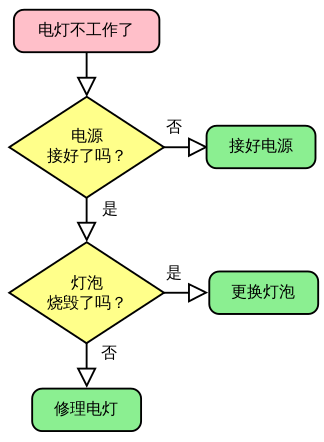
\includegraphics[width=0.9\textwidth]{c8.code.alg.png}
    \end{figure}
    \column{0.4\textwidth}
  \begin{block}{常见数据结构}
    \begin{itemize}
      \item 数组(Array)
      \item 堆栈(Stack)
      \item 队列(Queue)
      \item 链表(Linked List)
      \item 树(Tree)
      \item 图(Graph)
      \item 堆(Heap)
      \item 散列表(Hash)
    \end{itemize}
  \end{block}
\end{columns}
\end{frame}

\begin{frame}
  \frametitle{数据结构和算法 | 基因表达 | 简介}
  \begin{block}{生物学问题}
    特定环境条件下、特性类型细胞中,人类基因组中的每一个基因是否表达?
  \end{block}
  \pause
  \begin{block}{实验方法与数据处理}
    \begin{itemize}
      \item 基因芯片、RNA测序……
      \item 芯片:探针$\Rightarrow$基因;亮度$\Rightarrow$表达值
      \item 测序:reads $\Rightarrow$基因;reads数$\Rightarrow$表达值
      \item 其他:质量控制,标准化,基因注释,……
    \end{itemize}
  \end{block}
  \pause
  \begin{block}{最终数据}
    \begin{itemize}
      \item 所有基因(30000):基因名
      \item 表达基因(8000)的表达水平:具体数值
      \item 未表达基因(22000)的表达值:0
    \end{itemize}
  \end{block}
\end{frame}

\begin{frame}
  \frametitle{数据结构和算法 | 基因表达 | 芯片}
  \begin{figure}
    \centering
    \includegraphics[width=0.6\textwidth]{c8.code.chip.png}
  \end{figure}
\end{frame}

\begin{frame}
  \frametitle{数据结构和算法 | 基因表达 | RNA-Seq}
  \begin{figure}
    \centering
    \includegraphics[width=0.8\textwidth,height=0.8\textheight]{c8.code.rnaseq.jpg}
  \end{figure}
\end{frame}

\begin{frame}
  \frametitle{数据结构和算法 | 基因表达 | 数据结构 | 未排序数组}
  \begin{block}{具体实现}
    只在数组中存储表达基因(8000)的基因名,丢弃未表达基因的基因名
  \end{block}
  \pause
  \begin{block}{可能的问题}
    \begin{itemize}
      \item 查找表达基因:平均比较4000次
      \item 查找未表达基因:必须比较8000次
      \item 查找未研究的基因:未表达?未研究?
    \end{itemize}
  \end{block}
\end{frame}

\begin{frame}
  \frametitle{数据结构和算法 | 基因表达 | 数据结构 | 未排序数组}
  \begin{block}{改进方法}
    \begin{itemize}
      \item 把30000个基因全部存储到数组中
      \item 把表达值附加在基因名的后面
    \end{itemize}
  \end{block}
  \pause
  \begin{block}{存在的问题}
    \begin{itemize}
      \item 每次查询:平均比较15000次
      \item 分割基因名和表达值
    \end{itemize}
  \end{block}
\end{frame}

\begin{frame}
  \frametitle{数据结构和算法 | 基因表达 | 数据结构 | 排序数组}
  \begin{block}{具体实现}
    \begin{itemize}
      \item 把所有基因名按照字母顺序排序后存储到数组中
      \item 使用折半查找的算法进行查找
    \end{itemize}
  \end{block}
  \pause
  \begin{block}{优缺点}
    \begin{itemize}
      \item 优点:只需大约15次循环比较即可
      \item 缺点:需要首先对列表进行排序
      \item 缺点:添加新元素时稍显繁琐
    \end{itemize}
  \end{block}
\end{frame}

\begin{frame}
  \frametitle{数据结构和算法 | 基因表达 | 数据结构 | 散列}
  \begin{block}{具体实现}
    \begin{itemize}
      \item 基因名$\Rightarrow$散列的键
      \item 表达值$\Rightarrow$散列的值
    \end{itemize}
  \end{block}
  \pause
  \begin{block}{优缺点}
    \begin{itemize}
      \item 优点:查找速度通常比折半查找快
      \item 优点:可以明确知道要查找的基因是否在数据集中存在
      \item 优点:添加或删除元素时非常方便
      \item 缺点:其中的元素没有经过排序
    \end{itemize}
  \end{block}
\end{frame}

\begin{frame}
  \frametitle{数据结构和算法 | 基因表达 | 数据结构 | 比较}
  \begin{block}{未排序的数组}
    \begin{itemize}
      \item 需要遍历数组,速度很慢
      \item 必须要把基因名和表达值分割开来
    \end{itemize}
  \end{block}
  \pause
  \begin{block}{排序数组和折半查找}
    \begin{itemize}
      \item 查找速度大幅提升
      \item 必须对列表进行排序
      \item 不停的插入元素、重新排序会非常慢
    \end{itemize}
  \end{block}
  \pause
  \begin{block}{散列}
    \begin{itemize}
      \item 键:基因名;值:表达值
      \item 相比折半查找有优势:速度快,明确是否被定义,添加或删除元素不需重排序
      \item 缺点:其中元素没有被排序
    \end{itemize}
  \end{block}
\end{frame}

\begin{frame}
  \frametitle{数据结构和算法 | 基因表达 | \alert{总结}}
  \begin{block}{需求}
  \begin{itemize}
    \item<1-> 看看某个元素是否在数据集中,元素的顺序无所谓
    \item<2-> 数据集需要排序、相对快速的查找,不需要频繁添加或删减元素
    \item<3-> 不需要对元素排序,但需要快速找到最新添加的元素
    \item<4-> 不需要对元素排序,但需要添加元素、移除“最老”的元素
  \end{itemize}
  \end{block}
  \begin{block}{数据结构}
    \begin{itemize}
      \item<1-> 散列
      \item<2-> 排序数组结合折半查找
      \item<3-> 数组结合push和pop函数
      \item<4-> 数组结合push和shift函数
    \end{itemize}
  \end{block}
\end{frame}

\begin{frame}[fragile]
  \frametitle{数据结构和算法 | 折半查找}
\begin{lstlisting}[basicstyle=\small\tt]
# 折半查找(binary search)的伪代码
Given a sorted array, and an element:

Until you find the element or discover it's not there,

  Pick the midpoint of the array, $array[scalar(@array)/2]

  Compare your element with the element at the midpoint

  If that matches your element, you're done.

  Else, ignore the half of the array that your element is not in
}
\end{lstlisting}
\end{frame}

\begin{frame}
  \frametitle{数据结构和算法 | 折半查找}
  \begin{figure}
    \centering
    \includegraphics[width=0.55\textwidth]{c8.code.binary.search.01.jpg}
    \includegraphics[width=0.42\textwidth]{c8.code.binary.search.02.png}
  \end{figure}
\end{frame}

\begin{frame}[fragile]
  \frametitle{数据结构和算法 | 普通查找}
\begin{lstlisting}[basicstyle=\small\tt]
#!/usr/bin/perl

use strict;
use warnings;

my @numbers = map { $_ * 3 } ( 0 .. 1000000 );

sub search {
    my ( $numbers, $target ) = @_;
    for my $i ( 0 .. $#$numbers ) {
        return $i if $numbers->[$i] == $target;
    }
    return;
}

print search( \@numbers, 699 ), "\n";
print search( \@numbers, 28 ),  "\n";
\end{lstlisting}
\end{frame}

\begin{frame}[fragile]
  \frametitle{数据结构和算法 | 折半查找}
\begin{lstlisting}[basicstyle=\scriptsize\tt,numberstyle=\tiny]
#!/usr/bin/perl
use strict; use warnings;

my @numbers = map { $_ * 3 } ( 0 .. 1000000 );
sub search {
   my ( $numbers, $target ) = @_;
   return binary_search( $numbers, $target, 0, $#$numbers );
}
sub binary_search {
   my ( $numbers, $target, $low, $high ) = @_;
   return if $high < $low;
   my $middle = int( ( $low + $high ) / 2 );
   if ( $numbers->[$middle] > $target ) {
      return binary_search($numbers, $target, $low, $middle-1);
   }
   elsif ( $numbers->[$middle] < $target ) {
      return binary_search($numbers, $target, $middle+1, $high);
   }
   return $middle;
}
print search( \@numbers, 699 ), "\n";
print search( \@numbers, 28 ),  "\n";
\end{lstlisting}
\end{frame}

\begin{frame}[fragile]
  \frametitle{数据结构和算法 | \alert{比较与排序}}
\begin{lstlisting}[basicstyle=\small\tt]
# 两个字符串一样,返回0
'ZZZ' cmp 'ZZZ'

# 两个字符串按字母顺序排列,返回-1
'AAA' cmp 'ZZZ'

# 两个字符串按字母顺序的逆序排列,返回1
'ZZZ' cmp 'AAA'

# 按照字母顺序/逆序对由字符串构成的数组进行排序
@array = sort @array;
@array = sort { $a cmp $b } @array;
@array = sort { $b cmp $a } @array;

# 以升序/降序对由数字构成的数组进行排序:
@array = sort { $a <=> $b } @array;
@array = sort { $b <=> $a } @array;
\end{lstlisting}
\end{frame}

\begin{frame}[fragile]
  \frametitle{数据结构和算法 | \alert{散列操作}}
\begin{lstlisting}
# 查看某个散列值是否被定义
if ( defined $myhash{'mykey'} ) { ... }

# 对散列的键进行排序
@sorted_keys = sort keys %my_hash;

# 对散列的值进行排序
@sorted_values = sort values %my_hash;
\end{lstlisting}
\pause
\begin{block}{散列}
  \begin{itemize}
    \item Perl的内置数据类型,易使用、易编程
    \item 对于程序员来说,懒惰的方法通常是最有效的方法(节省编程的时间通常要比节省程序运行的时间更加重要一些)
  \end{itemize}
\end{block}
\end{frame}

\begin{frame}
  \frametitle{数据结构和算法 | 数据库}
  \begin{block}{数据库}
    数据库,简单来说可视为电子化的文件柜——存储电子文件的处所,用户可以对文件中的数据运行新增、截取、更新、删除等操作。适用于存储和访问海量数据。\\
    \vspace{0.2em}
    数据库指的是以一定方式储存在一起、能为多个用户共享、具有尽可能小的冗余度、与应用程序彼此独立的数据集合。
  \end{block}
  \pause
  \begin{block}{数据库管理系统}
    数据库管理系统(Database Management System,DBMS)是为管理数据库而设计的电脑软件系统,一般具有存储、截取、安全保障、备份等基础功能。\\
    \vspace{0.1em}
    数据库管理系统可以依据它所支持的数据库模型来作分类(关系式、XML),或依据所支持的电脑类型来作分类(服务器群集、移动电话),或依据所用查询语言来作分类(SQL、XQuery),或依据性能冲量重点来作分类(最大规模、最高运行速度),亦或其他的分类方式。不论使用哪种分类方式,一些DBMS能够跨类,例如,同时支持多种查询语言。
  \end{block}
\end{frame}

\begin{frame}
  \frametitle{数据结构和算法 | 数据库 | 关系数据库}
关系数据库(relational database),是建立在关系模型基础上的数据库,借助于集合代数等数学概念和方法来处理数据库中的数据。\alert{关系数据库是存储和提取海量数据最流行的方法。}\\
\vspace{1em}
\alert{关系数据库把数据组织成表格进行存储。}表是以\alert{行和列的形式}组织起来的数据的集合。一个数据库包括一个或多个表。例如,可能有一个有关作者信息的名为authors的表。每列都包含特定类型的信息,如作者的姓氏。每行都包含有关特定作者的所有信息:姓、名、住址等等。在关系型数据库当中一个表就是一个关系,一个关系数据库可以包含多个表。\\
\vspace{1em}
数据通常通过一种查询语言进行输入和提取,即\alert{结构化查询语言(SQL, Structured Query Language)语言}。SQL是1974年由Boyce和Chamberlin提出的一种介于关系代数与关系演算之间的结构化查询语言,是一个通用的、功能极强的关系型数据库语言。
\end{frame}

\begin{frame}
  \frametitle{数据结构和算法 | 数据库 | 关系数据库}
  \begin{figure}
    \centering
    \includegraphics[width=\textwidth]{c8.code.rd.01.png}
  \end{figure}
\end{frame}

\begin{frame}
  \frametitle{数据结构和算法 | 数据库 | DBI}
  The \href{http://dbi.perl.org/}{DBI(Perl's Database Interface)} is the standard database interface module for Perl. It defines a set of methods, variables and conventions that provide a consistent database interface independent of the actual database being used. 
\end{frame}

\begin{frame}
  \frametitle{数据结构和算法 | DBM}
  DBM(database management)是一种文件数据储存数据,由于采用散列结构进行链接,因此具有一些数据库的特点功能。与普通文本数据库相比,具有稳定、检索速度快和支持量大的优点。由于DBM是从Unix系统中移植来的,因此在Unix/linux系统中优点比较明显,而在NT系统中则不太理想,在NT中使用有时会令数据文件变得十分庞大。\\
  \vspace{1em}
  DBM数据库采用散列方式保存数据,并与散列结合使用。 
\end{frame}

\begin{frame}
  \frametitle{数据结构和算法 | DBM | Perl}
  \begin{block}{DBM}
    Perl中简单的、内置的一种方法,来存储散列数据
  \end{block}
  \pause
  \begin{block}{初始化}
    启动后,把一个散列“绑定”到计算机硬盘上的一个文件
  \end{block}
  \pause
  \begin{block}{使用}
    像使用散列一样使用它(查找,添加、删除……)
  \end{block}
  \pause
  \begin{block}{特色}
    \begin{itemize}
      \item 简单且非常有用的数据库
      \item 适用于键-值数据集
    \end{itemize}
  \end{block}
\end{frame}

\begin{frame}
  \frametitle{数据结构和算法 | DBM | Perl}
  \begin{block}{Problem}
    You want to create, populate, inspect, or delete values in a DBM database.
  \end{block}
  \pause
  \begin{block}{Solution}
    Use \textbf{dbmopen} or \textbf{tie} to open the database and make it accessible through a hash. Then use the hash as you normally would. When you’re done, call \textbf{dbmclose} or \textbf{untie}.
  \end{block}
\end{frame}

\begin{frame}
  \frametitle{数据结构和算法 | DBM | Perl}
  \begin{block}{Discussion}
    Accessing a database as a hash is powerful but easy, giving you a persistent hash that sticks around after the program using it has finished running. It's also much faster than loading in a new hash every time; even if the hash has a million entries, your program starts up virtually instantaneously.\\
    \vspace{0.5em}
    The program treats the database as though it were a normal hash. You can even call \textbf{keys} or \textbf{each} on it. Likewise, \textbf{exists} and \textbf{defined} are implemented for tied DBM hashes. Unlike a normal hash, a DBM hash does not distinguish between those two functions.
  \end{block}
\end{frame}

\begin{frame}[fragile]
  \frametitle{数据结构和算法 | DBM | Perl | \textcolor{gray}{dbmopen}}
\begin{lstlisting}
use DB_File;  # optional; overrides default
dbmopen %HASH, $FILENAME, 0666  # open database, accessed through %HASH
  or die "Can't open $FILENAME:$!\n";

$V = $HASH{$KEY};  # retrieve from database
$HASH{$KEY} = $VALUE;  # put value into database
if (exists $HASH{$KEY}) {  # check whether in database
  # ...
}
delete $HASH{$KEY};  # remove from database
dbmclose %HASH;  # close the database
\end{lstlisting}
\end{frame}

\begin{frame}[fragile]
  \frametitle{数据结构和算法 | DBM | Perl | tie}
\begin{lstlisting}
use DB_File;  # load database module

tie %HASH, "DB_File", $FILENAME  # open database, to be accessed
  or die "Can't open $FILENAME:$!\n";  # through %HASH

$V = $HASH{$KEY};  # retrieve from database
$HASH{$KEY} = $VALUE;  # put value into database
if (exists $HASH{$KEY}) {  # check whether in database
  # ...
}
delete $HASH{$KEY};  # delete from database
untie %HASH;  # close the database
\end{lstlisting}
\end{frame}

\begin{frame}[fragile]
  \frametitle{数据结构和算法 | DBM | Perl | 实例}
\begin{lstlisting}[basicstyle=\scriptsize\tt,numberstyle=\scriptsize]
#!/usr/bin/perl

use warnings; use strict;
use DB_File;

my ( %h, $k, $v );
unlink "fruit";

tie %h, "DB_File", "fruit", O_RDWR | O_CREAT, 0666, $DB_HASH or die "Cannot open file 'fruit': $!\n";

# Add a few key/value pairs to the file
$h{"apple"}  = "red"; $h{"orange"} = "orange";
$h{"banana"} = "yellow"; $h{"tomato"} = "red";
# Check for existence of a key
print "Banana Exists\n\n" if $h{"banana"};
# Delete a key/value pair.
delete $h{"apple"};
# print the contents of the file
while ( ( $k, $v ) = each %h ) { print "$k -> $v\n" }

untie %h;
\end{lstlisting}
\end{frame}

\begin{frame}[fragile]
  \frametitle{数据结构和算法 | DBM | Perl | 实例}
\begin{lstlisting}[basicstyle=\small\tt]
#!/usr/bin/perl
use warnings; use strict;
 
my %MYDB;
# 创建或打开DBM;如果是新建DBM,会自动生成mydb.dir和mydb.pag两个文件
dbmopen(%MYDB, "mydb", 0644)  or die "Can not access the database";

# 添加key/value对
$MYDB{name1} = "will1"; $MYDB{name2} = "will2";
# 读取内容
foreach my $key (keys %MYDB) {
  print "$key\t$MYDB{$key}\n";
}

# 关闭DBM
dbmclose(%MYDB) or die "Can not close database";
\end{lstlisting}
\end{frame}

\section{遗传密码}
\begin{frame}
  \frametitle{遗传密码 | 简介}
  遗传密码(genetic code)是一组规则,将DNA或mRNA序列以三个核苷酸为一组的密码子(codon)翻译为蛋白质的氨基酸序列,用于蛋白质合成。\\
  \vspace{1em}
  几乎所有的生物都使用同样的遗传密码,称为标准遗传密码;即使是非细胞结构的病毒,它们也是使用标准遗传密码。但是也有少数生物使用一些稍微不同的遗传密码。
\end{frame}

\begin{frame}
  \frametitle{遗传密码 | 简介}
  \begin{figure}
    \centering
    \includegraphics[width=0.65\textwidth]{c8.code.codon.01.png}
  \end{figure}
\end{frame}

\subsection{密码子翻译成氨基酸}
\begin{frame}
  \frametitle{遗传密码 | 密码子翻译}
  \begin{block}{生物学目的}
 把三个核苷酸的密码子翻译成氨基酸。 
  \end{block}
  \pause
  \begin{block}{程序实现}
    输入三字母的DNA密码子,返回一个单字母缩写表示的氨基酸。
  \end{block}
\end{frame}

\begin{frame}[fragile]
  \frametitle{遗传密码 | 密码子翻译}
\begin{lstlisting}[firstnumber=1,basicstyle=\footnotesize\tt,numberstyle=\scriptsize]
# codon2aa
#
# A subroutine to translate a DNA 3-character codon to an amino acid

sub codon2aa {
  my($codon) = @_;
          
     if ( $codon =~ /TCA/i ) { return 'S' } # Serine
  elsif ( $codon =~ /TCC/i ) { return 'S' } # Serine
  elsif ( $codon =~ /TCG/i ) { return 'S' } # Serine
  elsif ( $codon =~ /TCT/i ) { return 'S' } # Serine
  elsif ( $codon =~ /TTC/i ) { return 'F' } # Phenylalanine
  elsif ( $codon =~ /TTT/i ) { return 'F' } # Phenylalanine
  elsif ( $codon =~ /TTA/i ) { return 'L' } # Leucine
  elsif ( $codon =~ /TTG/i ) { return 'L' } # Leucine
\end{lstlisting}
\end{frame}

\begin{frame}[fragile]
  \frametitle{遗传密码 | 密码子翻译}
\begin{lstlisting}[firstnumber=16,basicstyle=\footnotesize\tt,numberstyle=\scriptsize]
  elsif ( $codon =~ /TAC/i ) { return 'Y' } # Tyrosine
  elsif ( $codon =~ /TAT/i ) { return 'Y' } # Tyrosine
  elsif ( $codon =~ /TAA/i ) { return '_' } # Stop
  elsif ( $codon =~ /TAG/i ) { return '_' } # Stop
  elsif ( $codon =~ /TGC/i ) { return 'C' } # Cysteine
  elsif ( $codon =~ /TGT/i ) { return 'C' } # Cysteine
  elsif ( $codon =~ /TGA/i ) { return '_' } # Stop
  elsif ( $codon =~ /TGG/i ) { return 'W' } # Tryptophan
  elsif ( $codon =~ /CTA/i ) { return 'L' } # Leucine
  elsif ( $codon =~ /CTC/i ) { return 'L' } # Leucine
  elsif ( $codon =~ /CTG/i ) { return 'L' } # Leucine
  elsif ( $codon =~ /CTT/i ) { return 'L' } # Leucine
  elsif ( $codon =~ /CCA/i ) { return 'P' } # Proline
  elsif ( $codon =~ /CCC/i ) { return 'P' } # Proline
  elsif ( $codon =~ /CCG/i ) { return 'P' } # Proline
  elsif ( $codon =~ /CCT/i ) { return 'P' } # Proline
  elsif ( $codon =~ /CAC/i ) { return 'H' } # Histidine
  elsif ( $codon =~ /CAT/i ) { return 'H' } # Histidine
\end{lstlisting}
\end{frame}

\begin{frame}[fragile]
  \frametitle{遗传密码 | 密码子翻译}
\begin{lstlisting}[firstnumber=34,basicstyle=\footnotesize\tt,numberstyle=\scriptsize]
  elsif ( $codon =~ /CAA/i ) { return 'Q' } # Glutamine
  elsif ( $codon =~ /CAG/i ) { return 'Q' } # Glutamine
  elsif ( $codon =~ /CGA/i ) { return 'R' } # Arginine
  elsif ( $codon =~ /CGC/i ) { return 'R' } # Arginine
  elsif ( $codon =~ /CGG/i ) { return 'R' } # Arginine
  elsif ( $codon =~ /CGT/i ) { return 'R' } # Arginine
  elsif ( $codon =~ /ATA/i ) { return 'I' } # Isoleucine
  elsif ( $codon =~ /ATC/i ) { return 'I' } # Isoleucine
  elsif ( $codon =~ /ATT/i ) { return 'I' } # Isoleucine
  elsif ( $codon =~ /ATG/i ) { return 'M' } # Methionine
  elsif ( $codon =~ /ACA/i ) { return 'T' } # Threonine
  elsif ( $codon =~ /ACC/i ) { return 'T' } # Threonine
  elsif ( $codon =~ /ACG/i ) { return 'T' } # Threonine
  elsif ( $codon =~ /ACT/i ) { return 'T' } # Threonine
  elsif ( $codon =~ /AAC/i ) { return 'N' } # Asparagine
  elsif ( $codon =~ /AAT/i ) { return 'N' } # Asparagine
  elsif ( $codon =~ /AAA/i ) { return 'K' } # Lysine
  elsif ( $codon =~ /AAG/i ) { return 'K' } # Lysine
\end{lstlisting}
\end{frame}

\begin{frame}[fragile]
  \frametitle{遗传密码 | 密码子翻译}
\begin{lstlisting}[firstnumber=52,basicstyle=\footnotesize\tt,numberstyle=\scriptsize]
  elsif ( $codon =~ /AGC/i ) { return 'S' } # Serine
  elsif ( $codon =~ /AGT/i ) { return 'S' } # Serine
  elsif ( $codon =~ /AGA/i ) { return 'R' } # Arginine
  elsif ( $codon =~ /AGG/i ) { return 'R' } # Arginine
  elsif ( $codon =~ /GTA/i ) { return 'V' } # Valine
  elsif ( $codon =~ /GTC/i ) { return 'V' } # Valine
  elsif ( $codon =~ /GTG/i ) { return 'V' } # Valine
  elsif ( $codon =~ /GTT/i ) { return 'V' } # Valine
  elsif ( $codon =~ /GCA/i ) { return 'A' } # Alanine
  elsif ( $codon =~ /GCC/i ) { return 'A' } # Alanine
  elsif ( $codon =~ /GCG/i ) { return 'A' } # Alanine
  elsif ( $codon =~ /GCT/i ) { return 'A' } # Alanine
  elsif ( $codon =~ /GAC/i ) { return 'D' } # Aspartic Acid
  elsif ( $codon =~ /GAT/i ) { return 'D' } # Aspartic Acid
\end{lstlisting}
\end{frame}

\begin{frame}[fragile]
  \frametitle{遗传密码 | 密码子翻译}
\begin{lstlisting}[firstnumber=66,basicstyle=\footnotesize\tt,numberstyle=\scriptsize]
  elsif ( $codon =~ /GAA/i ) { return 'E' } # Glutamic Acid
  elsif ( $codon =~ /GAG/i ) { return 'E' } # Glutamic Acid
  elsif ( $codon =~ /GGA/i ) { return 'G' } # Glycine
  elsif ( $codon =~ /GGC/i ) { return 'G' } # Glycine
  elsif ( $codon =~ /GGG/i ) { return 'G' } # Glycine
  elsif ( $codon =~ /GGT/i ) { return 'G' } # Glycine
  else {
    print STDERR "Bad codon \"$codon\"!!\n";
    exit;
  }
}
\end{lstlisting}
\end{frame}

\begin{frame}
  \frametitle{遗传密码 | 密码子翻译 | 总结}
  \begin{block}{优点}
    \begin{itemize}
      \item 代码清晰简单
      \item 排版布局美观
      \item 两者相得益彰,使整个翻译过程一目了然
    \end{itemize}
  \end{block}
  \pause
  \begin{block}{缺点}
    \begin{itemize}
      \item 大量的字符串比较
      \item 运行起来耗费时间
    \end{itemize}
  \end{block}
\end{frame}

\begin{frame}
  \frametitle{遗传密码 | 密码子翻译 | \alert{文件句柄}}
  \begin{block}{STDIN}
    \begin{itemize}
      \item 标准输入(默认键盘)
    \end{itemize}
  \end{block}
  \pause
  \begin{block}{STDOUT}
    \begin{itemize}
      \item 标准输出(默认屏幕)
      \item print默认使用STDOUT
      \item print可以使用一个文件句柄作为可选的参数
    \end{itemize}
  \end{block}
  \pause
  \begin{block}{STDERR}
    \begin{itemize}
      \item 标准错误输出(默认屏幕)
    \end{itemize}
  \end{block}
\end{frame}

\subsection{遗传密码的冗余性}
\begin{frame}
  \frametitle{遗传密码 | 冗余性}
  \begin{block}{碱基}
    4 = A + C + G + T/U
  \end{block}
  \pause
  \begin{block}{氨基酸}
    21 = 20(氨基酸) + 1(起始,同M) + 1(终止)
  \end{block}
  \pause
  \begin{block}{密码子}
    \begin{itemize}
      \item 每3个碱基组成一个密码子
      \item 一个密码子编码一种氨基酸
      \item 4x4x4=64 > 21
    \end{itemize}
  \end{block}
\end{frame}

\begin{frame}
  \frametitle{遗传密码 | 冗余性}
  \begin{figure}
    \centering
    \includegraphics[width=0.9\textwidth]{c8.code.codon.table.01.png}
  \end{figure}
\end{frame}

\begin{frame}
  \frametitle{遗传密码 | 冗余性}
  \begin{figure}
    \centering
    \includegraphics[width=0.9\textwidth]{c8.code.codon.table.02.png}
  \end{figure}
\end{frame}

\begin{frame}[fragile]
  \frametitle{遗传密码 | 冗余性}
\begin{lstlisting}[firstnumber=1,basicstyle=\scriptsize\tt,numberstyle=\tiny]
# codon2aa
#
# A subroutine to translate a DNA 3-character codon to an amino acid
#   Version 2

sub codon2aa {
  my($codon) = @_;
     
     if ( $codon =~ /GC./i )    { return 'A' } # Alanine
  elsif ( $codon =~ /TG[TC]/i ) { return 'C' } # Cysteine
  elsif ( $codon =~ /GA[TC]/i ) { return 'D' } # Aspartic Acid
  elsif ( $codon =~ /GA[AG]/i ) { return 'E' } # Glutamic Acid
  elsif ( $codon =~ /TT[TC]/i ) { return 'F' } # Phenylalanine
  elsif ( $codon =~ /GG./i )    { return 'G' } # Glycine
  elsif ( $codon =~ /CA[TC]/i ) { return 'H' } # Histidine
  elsif ( $codon =~ /AT[TCA]/i ){ return 'I' } # Isoleucine
  elsif ( $codon =~ /AA[AG]/i ) { return 'K' } # Lysine
  elsif ( $codon =~ /TT[AG]|CT./i ) { return 'L'} # Leucine
  elsif ( $codon =~ /ATG/i )    { return 'M' } # Methionine
  elsif ( $codon =~ /AA[TC]/i)  { return 'N' } # Asparagine
\end{lstlisting}
\end{frame}

\begin{frame}[fragile]
  \frametitle{遗传密码 | 冗余性}
\begin{lstlisting}[firstnumber=21,basicstyle=\scriptsize\tt,numberstyle=\tiny]
  elsif ( $codon =~ /CC./i )    { return 'P' } # Proline
  elsif ( $codon =~ /CA[AG]/i ) { return 'Q' } # Glutamine
  elsif ( $codon =~ /CG.|AG[AG]/i ) { return 'R' } # Arginine
  elsif ( $codon =~ /TC.|AG[TC]/i ) { return 'S' } # Serine
  elsif ( $codon =~ /AC./i )    { return 'T' } # Threonine
  elsif ( $codon =~ /GT./i )    { return 'V' } # Valine
  elsif ( $codon =~ /TGG/i )    { return 'W' } # Tryptophan
  elsif ( $codon =~ /TA[TC]/i ) { return 'Y' } # Tyrosine
  elsif ( $codon =~ /TA[AG]|TGA/i ) { return '_' } # Stop
  else {
    print STDERR "Bad codon \"$codon\"!!\n";
    exit;
  }
}
\end{lstlisting}
\end{frame}

\begin{frame}[fragile]
  \frametitle{遗传密码 | 冗余性 | 说明}
  \begin{block}{优势}
    \begin{itemize}
      \item 使用正则表达式展示了遗传密码的冗余性
      \item 氨基酸的单字母代码是按照字母顺序排列的
    \end{itemize}
  \end{block}
  \pause
  \begin{block}{\alert{正则表达式}}
    \begin{itemize}
      \item \verb|/[TC]/|:匹配T或者C
      \item \verb|/./|:匹配换行符以外的任意一个字符(此处为ACGT)
      \item \verb|/T/i|:不区分大小写,匹配T或者t
      \item \verb=/TC.|AG[TC]/=:匹配 \verb|/TC./|或者 \verb|/AG[TC]/|
      \item \verb=/TA[AG]|TGA/=:等同于 \verb=/T(A[AG]|GA)/=
    \end{itemize}
  \end{block}
\end{frame}

\subsection{使用散列表示遗传密码}
\begin{frame}[fragile]
  \frametitle{遗传密码 | 散列}
\begin{lstlisting}[firstnumber=1]
#
# codon2aa
#
# A subroutine to translate a DNA 3-character codon to an amino acid
#   Version 3, using hash lookup

sub codon2aa {
  my($codon) = @_;

  $codon = uc $codon;
\end{lstlisting}
\end{frame}

\begin{frame}[fragile]
  \frametitle{遗传密码 | 散列}
\begin{lstlisting}[firstnumber=12]
  my(%genetic_code) = (
	    
  'TCA' => 'S',    # Serine
  'TCC' => 'S',    # Serine
  'TCG' => 'S',    # Serine
  'TCT' => 'S',    # Serine
  'TTC' => 'F',    # Phenylalanine
  'TTT' => 'F',    # Phenylalanine
  'TTA' => 'L',    # Leucine
  'TTG' => 'L',    # Leucine
  'TAC' => 'Y',    # Tyrosine
  'TAT' => 'Y',    # Tyrosine
  'TAA' => '_',    # Stop
  'TAG' => '_',    # Stop
\end{lstlisting}
\end{frame}

\begin{frame}[fragile]
  \frametitle{遗传密码 | 散列}
\begin{lstlisting}[firstnumber=26,basicstyle=\scriptsize\tt,numberstyle=\tiny]
  'TGC' => 'C',    # Cysteine
  'TGT' => 'C',    # Cysteine
  'TGA' => '_',    # Stop
  'TGG' => 'W',    # Tryptophan
  'CTA' => 'L',    # Leucine
  'CTC' => 'L',    # Leucine
  'CTG' => 'L',    # Leucine
  'CTT' => 'L',    # Leucine
  'CCA' => 'P',    # Proline
  'CCC' => 'P',    # Proline
  'CCG' => 'P',    # Proline
  'CCT' => 'P',    # Proline
  'CAC' => 'H',    # Histidine
  'CAT' => 'H',    # Histidine
  'CAA' => 'Q',    # Glutamine
  'CAG' => 'Q',    # Glutamine
  'CGA' => 'R',    # Arginine
  'CGC' => 'R',    # Arginine
  'CGG' => 'R',    # Arginine
  'CGT' => 'R',    # Arginine
\end{lstlisting}
\end{frame}

\begin{frame}[fragile]
  \frametitle{遗传密码 | 散列}
\begin{lstlisting}[firstnumber=46,basicstyle=\scriptsize\tt,numberstyle=\tiny]
  'ATA' => 'I',    # Isoleucine
  'ATC' => 'I',    # Isoleucine
  'ATT' => 'I',    # Isoleucine
  'ATG' => 'M',    # Methionine
  'ACA' => 'T',    # Threonine
  'ACC' => 'T',    # Threonine
  'ACG' => 'T',    # Threonine
  'ACT' => 'T',    # Threonine
  'AAC' => 'N',    # Asparagine
  'AAT' => 'N',    # Asparagine
  'AAA' => 'K',    # Lysine
  'AAG' => 'K',    # Lysine
  'AGC' => 'S',    # Serine
  'AGT' => 'S',    # Serine
  'AGA' => 'R',    # Arginine
  'AGG' => 'R',    # Arginine
  'GTA' => 'V',    # Valine
  'GTC' => 'V',    # Valine
  'GTG' => 'V',    # Valine
  'GTT' => 'V',    # Valine
\end{lstlisting}
\end{frame}

\begin{frame}[fragile]
  \frametitle{遗传密码 | 散列}
\begin{lstlisting}[firstnumber=66,basicstyle=\footnotesize\tt,numberstyle=\scriptsize]
  'GCA' => 'A',    # Alanine
  'GCC' => 'A',    # Alanine
  'GCG' => 'A',    # Alanine
  'GCT' => 'A',    # Alanine
  'GAC' => 'D',    # Aspartic Acid
  'GAT' => 'D',    # Aspartic Acid
  'GAA' => 'E',    # Glutamic Acid
  'GAG' => 'E',    # Glutamic Acid
  'GGA' => 'G',    # Glycine
  'GGC' => 'G',    # Glycine
  'GGG' => 'G',    # Glycine
  'GGT' => 'G',    # Glycine
  );

  if(exists $genetic_code{$codon}) {
    return $genetic_code{$codon};
  }else{
    print STDERR "Bad codon \"$codon\"!!\n";
    exit;
  }
}
\end{lstlisting}
\end{frame}

\begin{frame}[fragile]
  \frametitle{遗传密码 | 散列 | \alert{说明}}
  \begin{block}{代码解释}
  \begin{itemize}
    \item \verb|uc $codon|:把输入的参数转换为大写(子程序就可以同时处理大小写了)
    \item \verb|exists $genetic_code{$condon}|:散列中存在 \verb|$codon|这个键就返回true,否则返回false
  \end{itemize}
  \end{block}
  \pause
  \begin{block}{补充说明}
    \begin{itemize}
      \item 散列的键必须是简单的标量值,不能使用正则表达式,不能使用字符集
      \item 使用子程序(做成“黑盒子”)对程序进行模块化组织
      \item 把codon2aa这个子程序放到BeginPerlBioinfo.pm模块文件中备用
    \end{itemize}
  \end{block}
\end{frame}

\section{DNA翻译成蛋白质}
\begin{frame}
  \frametitle{DNA翻译成蛋白质 | 目的}
  \begin{block}{目的}
    使用子程序codon2aa把整个DNA序列翻译成蛋白质。
  \end{block}
  \begin{figure}
    \centering
    \includegraphics[width=0.9\textwidth]{c8.code.translation.01.jpg}
  \end{figure}
\end{frame}

\begin{frame}[fragile]
  \frametitle{DNA翻译成蛋白质 | 程序8.1.1}
\begin{lstlisting}[firstnumber=1]
#!/usr/bin/perl -w
# Example 8-1   Translate DNA into protein

use strict;
use warnings;
use BeginPerlBioinfo;     # see Chapter 6 about this module

# Initialize variables
my $dna = 'CGACGTCTTCGTACGGGACTAGCTCGTGTCGGTCGC';
my $protein = '';
my $codon;
\end{lstlisting}
\end{frame}

\begin{frame}[fragile]
  \frametitle{DNA翻译成蛋白质 | 程序8.1.2}
\begin{lstlisting}[firstnumber=13]
# Translate each three-base codon into an amino acid, and append to a protein 
for(my $i=0; $i < (length($dna) - 2) ; $i += 3) {
    $codon = substr($dna,$i,3);
    $protein .= codon2aa($codon);
}

print "I translated the DNA\n\n$dna\n\n  into the protein\n\n$protein\n\n";

exit;
\end{lstlisting}
\end{frame}

\begin{frame}[fragile]
  \frametitle{DNA翻译成蛋白质 | 程序8.1 | 输出}
\begin{lstlisting}
I translated the DNA

CGACGTCTTCGTACGGGACTAGCTCGTGTCGGTCGC

  into the protein

RRLRTGLARVGR
\end{lstlisting}
\end{frame}

\begin{frame}[fragile]
  \frametitle{DNA翻译成蛋白质 | 程序8.1 | \alert{循环}}
\begin{lstlisting}
for (my $i = 0; $i < (length($dna) - 2); $i += 3) {
\end{lstlisting}
\pause
\begin{block}{解释}
  \begin{itemize}
    \item \verb|my $i=0|:初始化计数器,限定作用域
    \item \verb|$i<(length($dna)-2)|:判断是否继续翻译,密码子长度为3,DNA序列长 \verb|length|,其中的碱基索引从0到 \verb|length-1|
    \item \verb|$i+=3|:计数器递增,一次处理3个碱基
  \end{itemize}
\end{block}
\end{frame}

\begin{frame}[fragile]
  \frametitle{DNA翻译成蛋白质 | 程序8.1 | \alert{提取密码子}}
\begin{lstlisting}
$codon = substr ($dna, $i, 3);
\end{lstlisting}
\pause
\begin{block}{解释}
  \begin{itemize}
    \item 从字符串 \verb|$dna|的位置 \verb|$i|开始向后提取3个字符
    \item 把提取的子字符串保存到变量 \verb|$codon|中
  \end{itemize}
\end{block}
\end{frame}

\begin{frame}
  \frametitle{DNA翻译成蛋白质 | 程序8.1 | 转换成子程序}
  \begin{block}{基本要求}
  \begin{itemize}
    \item 输入:包含DNA的参数
    \item 返回:翻译后的肽链
  \end{itemize}
  \end{block}
  \pause
  \begin{block}{问题简化}
    \begin{itemize}
      \item 翻译整段DNA(不需要提供指定起始和终止位点的参数)
      \item 移除不适合于子程序的print语句
    \end{itemize}
  \end{block}
\end{frame}

\begin{frame}[fragile]
  \frametitle{DNA翻译成蛋白质 | \alert{子程序}}
\begin{lstlisting}[firstnumber=1]
# dna2peptide 
#
# A subroutine to translate DNA sequence into a peptide

sub dna2peptide {

  my($dna) = @_;

  use strict;
  use warnings;
  use BeginPerlBioinfo;     # see Chapter 6 about this module
\end{lstlisting}
\end{frame}

\begin{frame}[fragile]
  \frametitle{DNA翻译成蛋白质 | \alert{子程序}}
\begin{lstlisting}[firstnumber=13]
  # Initialize variables
  my $protein = '';

  # Translate each three-base codon to an amino acid, and append to a protein 
  for(my $i=0; $i < (length($dna) - 2) ; $i += 3) {
    $protein .= codon2aa( substr($dna,$i,3));
  }

  return $protein;
}
\end{lstlisting}
\end{frame}

\begin{frame}[fragile]
  \frametitle{DNA翻译成蛋白质 | 子程序 | \alert{说明}}
  \begin{block}{易读 vs. 速度}
    \begin{itemize}
      \item 使用 \verb|$codon|中间变量:更加易读
      \item 不使用 \verb|$codon|中间变量:避免字符串的复制,提高运行速度
      \item 当程序本身的易读性降低时,补充注释进行说明
    \end{itemize}
  \end{block}
  \pause
  \begin{block}{use}
    \begin{itemize}
      \item 可以在子程序中使用use载入模块
      \item 子程序的use可以和主程序的use存在冗余
      \item Perl只会载入模块一次
      \item 子程序中载入模块有一定的优势(主程序中没有载入这些模块时)
    \end{itemize}
  \end{block}
\end{frame}

\section{读取FASTA格式的DNA}
\subsection{序列格式}
\begin{frame}
  \frametitle{读取FASTA格式的DNA | 序列格式}
  \begin{itemize}
    \item Plain sequence format
    \item FASTA format
    \item GenBank format
    \item EMBL format
    \item GCG format
    \item GCG-RSF (rich sequence format)
    \item IG format
  \end{itemize}
\end{frame}

\begin{frame}
  \frametitle{读取FASTA格式的DNA | 序列格式 | \alert{Plain}}
  \begin{figure}
    \centering
    \includegraphics[width=\textwidth]{c8.code.format.plain.png}
  \end{figure}
\end{frame}

\begin{frame}
  \frametitle{读取FASTA格式的DNA | 序列格式 | \alert{FASTA}}
  \begin{figure}
    \centering
    \includegraphics[width=\textwidth]{c8.code.format.fasta.png}
  \end{figure}
\end{frame}

\begin{frame}
  \frametitle{读取FASTA格式的DNA | 序列格式 | \alert{GenBank}}
  \begin{figure}
    \centering
    \includegraphics[width=\textwidth]{c8.code.format.genbank.png}
  \end{figure}
\end{frame}

\begin{frame}
  \frametitle{读取FASTA格式的DNA | 序列格式 | \alert{EMBL}}
  \begin{figure}
    \centering
    \includegraphics[width=\textwidth]{c8.code.format.embl.png}
  \end{figure}
\end{frame}

\begin{frame}
  \frametitle{读取FASTA格式的DNA | 序列格式 | GCG}
  \begin{figure}
    \centering
    \includegraphics[width=\textwidth]{c8.code.format.gcg.png}
  \end{figure}
\end{frame}

\begin{frame}
  \frametitle{读取FASTA格式的DNA | 序列格式 | IG}
  \begin{figure}
    \centering
    \includegraphics[width=\textwidth]{c8.code.format.ig.png}
  \end{figure}
\end{frame}

\subsection{读取FASTA文件的思路}
\begin{frame}
  \frametitle{读取FASTA文件 | \alert{策略}}
  \begin{block}{读取文件的两种策略}
    \begin{enumerate}
      \item 从打开的文件中一次读入一行,边读入、边处理
	\begin{itemize}
	  \item 大文件
	  \item 寻找小的信息片段
	\end{itemize}
      \item 一次性把整个文件都读入到数组中,然后对数组进行操作
	\begin{itemize}
	  \item 中、小文件
	  \item 容易遍历整个数据进行操作
	\end{itemize}
    \end{enumerate}
  \end{block}
\end{frame}

\begin{frame}
  \frametitle{读取FASTA文件 | 思路}
  \begin{block}{要求}
    \begin{itemize}
      \item 输入:FASTA文件的文件名参数
      \item 返回:FASTA文件中的序列数据
    \end{itemize}
  \end{block}
  \pause
  \begin{block}{思路}
    \begin{itemize}
      \item 一个子程序:打开、读取FATSA文件并提取序列数据
      \item 两个子程序
	\begin{enumerate}
	  \item 第一个子程序:打开并读取文件
	  \item 第二个子程序:提取序列数据
	\end{enumerate}
    \end{itemize}
  \end{block}
\end{frame}

\begin{frame}[fragile]
  \frametitle{读取FASTA文件 | 两个子程序 | 伪代码 | 处理文件}
\begin{lstlisting}
subroutine get data from a file

  argument = filename

  open file
    if can't open, print error message and exit

  read in data and 

  return @data
}
\end{lstlisting}
\end{frame}

\begin{frame}[fragile]
  \frametitle{读取FASTA文件 | 两个子程序 | 伪代码 | 提取序列}
\begin{lstlisting}[basicstyle=\small\tt]
Subroutine extract sequence data from fasta file

  argument = array of file data in fasta format

    Discard all header lines
    (and blank and comment lines for good measure)
    If first character of first line is >, discard it

  Read in the rest of the file, join in a scalar,
    edit out nonsequence data

  return sequence
}
\end{lstlisting}
\end{frame}

\begin{frame}
  \frametitle{读取FASTA文件 | \alert{读取失败}}
  如果文件不能被读取,可能的处理方法:
  \begin{itemize}
    \item 退出程序:比较极端
    \item 向用户询问文件名:人性化,不利于自动化
    \item 使用默认的文件:人性化,自动化
    \item 返回false(空数组):容易和空文件相混淆
    \item 其他处理方法:返回undefined
  \end{itemize}
\end{frame}

\subsection{读取FASTA文件的子程序}
\begin{frame}[fragile]
  \frametitle{读取FASTA文件 | 子程序}
\begin{lstlisting}[firstnumber=1,basicstyle=\footnotesize\tt,numberstyle=\scriptsize]
# get_file_data
# A subroutine to get data from a file given its filename

sub get_file_data {
  my($filename) = @_;
  use strict;
  use warnings;
  # Initialize variables
  my @filedata = ( );
  unless( open(GET_FILE_DATA, $filename) ) {
    print STDERR "Cannot open file \"$filename\"\n\n";
    exit;
  }
  @filedata = <GET_FILE_DATA>;
  close GET_FILE_DATA;
  return @filedata;
}
\end{lstlisting}
\end{frame}

\begin{frame}[fragile]
  \frametitle{读取FASTA文件 | 子程序}
\begin{lstlisting}[firstnumber=31,basicstyle=\footnotesize\tt,numberstyle=\scriptsize]
# extract_sequence_from_fasta_data: A subroutine to extract FASTA sequence data from an array
sub extract_sequence_from_fasta_data {
  my(@fasta_file_data) = @_;
  use strict; use warnings;
  my $sequence = ''; # Declare and initialize variables
  foreach my $line (@fasta_file_data) {
    # discard blank line
    if ($line =~ /^\s*$/) { next;
    # discard comment line 
    } elsif($line =~ /^\s*#/) { next;
    # discard fasta header line
    } elsif($line =~ /^>/) { next;
    # keep line, add to sequence string
    } else { $sequence .= $line; }
  }
  # remove non-sequence data (in this case, whitespace) from $sequence string
  $sequence =~ s/\s//g; return $sequence;
}
\end{lstlisting}
\end{frame}

\begin{frame}[fragile]
  \frametitle{读取FASTA文件 | 子程序 | \alert{说明}}
\begin{lstlisting}
# 使用my声明循环中使用的变量
foreach my $line (@fasta_file_data) {

# 匹配只有/没有空白的空行
if ($line =~ /^\s*$/) {

# 匹配注释行
} elsif($line =~ /^\s*#/) {

# 匹配FASTA标题行
} elsif($line =~ /^>/) {

# 删除空白字符(含换行符)
$sequence =~ s/\s//g;
\end{lstlisting}
\end{frame}

\subsection{输出格式化的序列数据}
\begin{frame}
  \frametitle{格式化序列数据 | 任务}
  \begin{block}{格式化序列数据}
    \begin{itemize}
      \item 目的:把序列数据格式化成适当长度
      \item 输入:序列和行的长度两个参数
      \item 输出:按指定要求格式化后的序列数据
    \end{itemize}
  \end{block}
\end{frame}

\begin{frame}[fragile]
  \frametitle{格式化序列数据 | \alert{子程序}}
\begin{lstlisting}
# print_sequence
# A subroutine to format and print sequence data 

sub print_sequence {
  my($sequence, $length) = @_;
  use strict;
  use warnings;
  # Print sequence in lines of $length
  for ( my $pos = 0 ; $pos < length($sequence) ; $pos += $length ) {
    print substr($sequence, $pos, $length), "\n";
  }
}
\end{lstlisting}
\end{frame}

\subsection{读取FASTA文件的主程序}
\begin{frame}[fragile]
  \frametitle{读取FASTA文件 | 程序8.2.1}
\begin{lstlisting}[firstnumber=1]
#!/usr/bin/perl -w
# Example 8-2   Read a fasta file and extract the sequence data

use strict;
use warnings;
use BeginPerlBioinfo;     # see Chapter 6 about this module

# Declare and initialize variables
my @file_data = (  );
my $dna = '';
\end{lstlisting}
\end{frame}

\begin{frame}[fragile]
  \frametitle{读取FASTA文件 | 程序8.2.1}
\begin{lstlisting}[firstnumber=12]
# Read in the contents of the file "sample.dna"
@file_data = get_file_data("sample.dna");

# Extract the sequence data from the contents of the file "sample.dna"
$dna = extract_sequence_from_fasta_data(@file_data);

# Print the sequence in lines 25 characters long
print_sequence($dna, 25);

exit;
\end{lstlisting}
\end{frame}

\begin{frame}[fragile]
  \frametitle{读取FASTA文件 | 程序8.2 | 输出}
\begin{lstlisting}
agatggcggcgctgaggggtcttgg
gggctctaggccggccacctactgg
tttgcagcggagacgacgcatgggg
cctgcgcaataggagtacgctgcct
gggaggcgtgactagaagcggaagt
...
ccaacagcagccacagccatcacag
aagttagggcgcatccgtgaagatg
agggggcagtggcgtcatcaacagt
caaggagcctcctgaggctacagcc
acacctgagccactctcagatgagg
accta
\end{lstlisting}
\end{frame}

\subsection{DNA翻译成蛋白质的主程序}
\begin{frame}[fragile]
  \frametitle{DNA翻译成蛋白质 | 程序8.3.1}
\begin{lstlisting}[firstnumber=1]
#!/usr/bin/perl -w
# Example 8-3   Read a fasta file and extract the DNA sequence data
# Translate it to protein and print it out in 25-character-long lines

use strict;
use warnings;
use BeginPerlBioinfo;     # see Chapter 6 about this module

# Initialize variables
my @file_data = (  );
my $dna = '';
my $protein = '';
\end{lstlisting}
\end{frame}

\begin{frame}[fragile]
  \frametitle{DNA翻译成蛋白质 | 程序8.3.1}
\begin{lstlisting}[firstnumber=13]
# Read in the contents of the file "sample.dna"
@file_data = get_file_data("sample.dna");

# Extract the sequence data from the contents of the file "sample.dna"
$dna = extract_sequence_from_fasta_data(@file_data);

# Translate the DNA to protein
$protein = dna2peptide($dna);

# Print the sequence in lines 25 characters long
print_sequence($protein, 25);

exit;
\end{lstlisting}
\end{frame}

\begin{frame}[fragile]
  \frametitle{DNA翻译成蛋白质 | 程序8.3 | 输出}
\begin{lstlisting}[firstnumber=1]
RWRR_GVLGALGRPPTGLQRRRRMG
PAQ_EYAAWEA_LEAEVVVGAFATA
WDAAEWSVQVRGSLAGVVRECAGSG
DMEGDGSDPEPPDAGEDSKSENGEN
APIYCICRKPDINCFMIGCDNCNEW
FHGDCIRITEKMAKAIREWYCRECR
EKDPKLEIRYRHKKSRERDGNERDS
SEPRDEGGGRKRPVPDPDLQRRAGS
GTGVGAMLARGSASPHKSSPQPLVA
TPSQHHQQQQQQIKRSARMCGECEA
CRRTEDCGHCDFCRDMKKFGGPNKI
RQKCRLRQCQLRARESYKYFPSSLS
PVTPSESLPRPRRPLPTQQQPQPSQ
KLGRIREDEGAVASSTVKEPPEATA
TPEPLSDEDL
\end{lstlisting}
\end{frame}

\section{阅读框}
\subsection{简介}
\begin{frame}
  \frametitle{阅读框 | 阅读框架}
  阅读框架(reading frame)是指RNA或DNA中,一组连续且不重复的3核苷酸密码子。每一条mRNA共有3种可能的阅读框架,而双股的DNA则每股各3种,共6种阅读框架。\\
  \vspace{1em}
  同一序列具有多种阅读框架的现象使重叠基因(overlapping genes)可能存在,已知常见于某些细菌与病毒。至于人类细胞中则较少见。
\end{frame}

\begin{frame}
  \frametitle{阅读框 | 阅读框架 | \alert{6种}}
  \begin{figure}
    \centering
    \includegraphics[width=0.7\textwidth]{c8.code.orf.01.jpg}
  \end{figure}
\end{frame}

\begin{frame}
  \frametitle{阅读框 | \alert{开放阅读框}}
  开放阅读框(open reading frame,ORF)是指在给定的阅读框架中,不包含终止密码子的一串序列。这段序列是生物个体的基因组中,可能作为蛋白质编码序列的部分。基因中的ORF包含并位于开始编码与终止编码之间。\\
  \vspace{1em}
  由于一段DNA或RNA序列有多种不同读取方式,因此可能同时存在许多不同的开放阅读框架。\\
  \vspace{1em}
  开放阅读框是判断DNA序列中存在基因的一个重要依据;基因识别程序需要进行开放阅读框的分析。
\end{frame}

\begin{frame}
  \frametitle{阅读框 | 动手之前的思考}
  \begin{block}{基本思想}
    \begin{itemize}
      \item 一切高大上的问题/任务都是纸老虎
    \end{itemize}
  \end{block}
  \pause
  \begin{block}{解决思路}
    \begin{itemize}
      \item 四处寻找已经写好的、可以完成该任务的(子)程序/工具
      \item 充分利用自己收集的子程序库
	\begin{itemize}
	  \item 有哪些相关的子程序可以直接使用
	  \item 有哪些相关的子程序需要进行修改/扩展
	  \item 还缺少哪些子程序需要编写添加
	\end{itemize}
    \end{itemize}
  \end{block}
\end{frame}

\begin{frame}
  \frametitle{阅读框 | 子程序库}
  \begin{block}{已有的子程序}
    \begin{itemize}
      \item get\_file\_data:打开读取文件
      \item extract\_sequence\_from\_fasta\_data:提取FASTA文件中的序列
      \item dna2peptide:把DNA翻译成多肽
	\begin{itemize}
	  \item codon2aa:把密码子翻译成氨基酸
	\end{itemize}
      \item print\_sequence:输出格式化的序列
    \end{itemize}
  \end{block}
  \pause
  \begin{block}{尚缺的子程序}
    \begin{itemize}
      \item revcom:计算反向互补序列
      \item translate\_frame:翻译DNA的指定区间
    \end{itemize}
  \end{block}
\end{frame}

\subsection{翻译阅读框}
\begin{frame}[fragile]
  \frametitle{阅读框 | 翻译 | 反向互补 | 子程序}
\begin{lstlisting}
# revcom 
# A subroutine to compute the reverse complement of DNA sequence
sub revcom {
  my($dna) = @_;

  # First reverse the sequence
  my($revcom) = reverse($dna);

  # Next, complement the sequence, dealing with upper and lower case
  # A->T, T->A, C->G, G->C
  $revcom =~ tr/ACGTacgt/TGCAtgca/;

  return $revcom;
}
\end{lstlisting}
\end{frame}

\begin{frame}[fragile]
  \frametitle{阅读框 | 翻译 | 指定区间 | 伪代码}
\begin{lstlisting}[basicstyle=\footnotesize\tt,numberstyle=\scriptsize]
Given DNA sequence

subroutine translate_frame ( DNA, start, end )

  return dna2peptide( substr( DNA, start, end - start + 1 ) )
}
\end{lstlisting}
\pause
\begin{lstlisting}[basicstyle=\footnotesize\tt,numberstyle=\scriptsize]
Given DNA sequence

subroutine translate_frame ( DNA, start, end )

  # start and end are numbering the sequence from 1 to length
  return dna2peptide( substr( DNA, start - 1, end - start + 1 ) )
}
\end{lstlisting}
\end{frame}

\begin{frame}[fragile]
  \frametitle{阅读框 | 翻译 | 指定区间 | \alert{索引}}
  \begin{block}{两种索引}
    \begin{itemize}
      \item Perl的处理方式:从0开始
      \item 生物学家的处理方式:从1开始
    \end{itemize}
  \end{block}
  \pause
  \begin{block}{推荐策略}
    \begin{itemize}
      \item 面向程序:以0起始的索引方式(计算简便)
      \item 面向用户:以1起始的索引方式(人性化)
    \end{itemize}
  \end{block}
\end{frame}

\begin{frame}[fragile]
  \frametitle{阅读框 | 翻译 | 指定区间 | \alert{子程序}}
\begin{lstlisting}[basicstyle=\footnotesize\tt,numberstyle=\scriptsize]
# translate_frame
# A subroutine to translate a frame of DNA

sub translate_frame {
  my($seq, $start, $end) = @_;
  #my $protein;

  # To make the subroutine easier to use, you won't need to specify the end point--it will just go to the end of the sequence by default.
  unless($end) {
    $end = length($seq);
  }

  # Finally, calculate and return the translation
  return dna2peptide ( substr ( $seq, $start - 1, $end -$start + 1 ) );
}
\end{lstlisting}
\end{frame}

\begin{frame}[fragile]
  \frametitle{阅读框 | 翻译 | 程序8.4.1}
\begin{lstlisting}[firstnumber=1]
#!/usr/bin/perl -w
# Example 8-4   Translate a DNA sequence in all six reading frames

use strict;
use warnings;
use BeginPerlBioinfo;     # see Chapter 6 about this module

# Initialize variables
my @file_data = (  );
my $dna = '';
my $revcom = '';
my $protein = '';
\end{lstlisting}
\end{frame}

\begin{frame}[fragile]
  \frametitle{阅读框 | 翻译 | 程序8.4.2}
\begin{lstlisting}[firstnumber=14,basicstyle=\small\tt,numberstyle=\footnotesize]
# Read in the contents of the file "sample.dna"
@file_data = get_file_data("sample.dna");

# Extract the sequence data from the contents of the file "sample.dna"
$dna = extract_sequence_from_fasta_data(@file_data);

# Translate the DNA to protein in six reading frames
#   and print the protein in lines 70 characters long
print "\n -------Reading Frame 1--------\n\n";
$protein = translate_frame($dna, 1);
print_sequence($protein, 70);
\end{lstlisting}
\end{frame}

\begin{frame}[fragile]
  \frametitle{阅读框 | 翻译 | 程序8.4.3}
\begin{lstlisting}[firstnumber=26]
print "\n -------Reading Frame 2--------\n\n";
$protein = translate_frame($dna, 2);
print_sequence($protein, 70);

print "\n -------Reading Frame 3--------\n\n";
$protein = translate_frame($dna, 3);
print_sequence($protein, 70);
\end{lstlisting}
\end{frame}

\begin{frame}[fragile]
  \frametitle{阅读框 | 翻译 | 程序8.4.4}
\begin{lstlisting}[firstnumber=34,basicstyle=\footnotesize\tt,numberstyle=\scriptsize]
# Calculate reverse complement
$revcom = revcom($dna);

print "\n -------Reading Frame 4--------\n\n";
$protein = translate_frame($revcom, 1);
print_sequence($protein, 70);

print "\n -------Reading Frame 5--------\n\n";
$protein = translate_frame($revcom, 2);
print_sequence($protein, 70);

print "\n -------Reading Frame 6--------\n\n";
$protein = translate_frame($revcom, 3);
print_sequence($protein, 70);

exit;
\end{lstlisting}
\end{frame}

\begin{frame}[fragile]
  \frametitle{阅读框 | 翻译 | 程序8.4 | 输出}
\begin{lstlisting}[language=,basicstyle=\tiny\tt,numberstyle=\tiny]
 -------Reading Frame 1--------

RWRR_GVLGALGRPPTGLQRRRRMGPAQ_EYAAWEA_LEAEVVVGAFATAWDAAEWSVQVRGSLAGVVRE
CAGSGDMEGDGSDPEPPDAGEDSKSENGENAPIYCICRKPDINCFMIGCDNCNEWFHGDCIRITEKMAKA
IREWYCRECREKDPKLEIRYRHKKSRERDGNERDSSEPRDEGGGRKRPVPDPDLQRRAGSGTGVGAMLAR
GSASPHKSSPQPLVATPSQHHQQQQQQIKRSARMCGECEACRRTEDCGHCDFCRDMKKFGGPNKIRQKCR
LRQCQLRARESYKYFPSSLSPVTPSESLPRPRRPLPTQQQPQPSQKLGRIREDEGAVASSTVKEPPEATA
TPEPLSDEDL

...

-------Reading Frame 6--------

GPHLRVAQVWL_PQEAP_LLMTPLPPHLHGCALTSVMAVAAVGWAVAGGALAGTLRASLVRARKGSTCTI
PGPAAGTGAAGTSAGSCWGPRTSSCPDRNHSDHSPQCADMPHTHHTCGLTV_SAAAAAGDAGWVWPPRAA
ERICGAKQSPEQAWPQPLSLTLPGAAGLDQGQASCALHPHPGAHCCPAHCHPAPVTSCADSESLAWGLSL
CTPDSTTPGWPWPSSQ_SGCSPHGTTHCSCHTRS_SS_CPVCGRCSRWAHSPHSRTCCPPRHLEALGLNH
LPPYLRSRRTPSRPPPATREPAQTTRRRPRRLQRRPQLLPLLVTPPRQRTPIAQAPCVVSAANQ_VAGLE
PPRPLSAAI
\end{lstlisting}
\end{frame}

\section{回顾和总结}
\subsection{总结}
\begin{frame}
  \frametitle{遗传密码 | 总结}
  \begin{block}{知识点}
    \begin{itemize}
      \item 散列:键,值,初始化,检查定义/存在,排序,……
      \item Perl中的数据类型:标量变量,数组,散列
      \item 正则表达式:元字符,字符集,修饰符,择一匹配
      \item 序列格式:plain,FASTA,GenBank,EMBL,……
      \item Perl读取文件:两种策略,读取失败的处理方法
      \item 阅读框:6种框架,开放阅读框
      \item 其他:数据结构,比较排序,文件句柄,循环,子字符串提取,索引,……
    \end{itemize}
  \end{block}
  \pause
  \begin{block}{技能}
    \begin{itemize}
      \item 熟练使用Perl中的散列
      \item 熟练使用Perl读取文件
      \item 能编写把DNA翻译成蛋白质的Perl程序
    \end{itemize}
  \end{block}
\end{frame}

\subsection{思考题}
\begin{frame}
  \frametitle{遗传密码 | 思考题}
  \begin{enumerate}
    \item 比较Perl的三种常见数据类型。
    \item 如何获取散列中的所有键/值?
    \item 如何对字符串/数字进行正序/逆序的排序?
    \item 举例说明不同任务下数据结构的选择。
    \item 如何使用正则表达式表征密码子?
    \item 列举并举例说明常见的序列格式。
    \item 比较读取文件的两种策略。
    \item 举例说明6种阅读框。
    \item 比较两种不同的索引方式。
    \item 举例说明子程序的使用。
  \end{enumerate}
\end{frame}

\begin{frame}
  \frametitle{下节预告}
  \begin{block}{计算机}
    回顾正则表达式的相关知识:元字符,字符集,量词,修饰符,……
  \end{block}
  \begin{block}{生物学}
    回顾限制性核酸内切酶的相关知识:定义,分类,特点,……
  \end{block}
\end{frame}

\section{扩展知识}
\subsection{Perl里面的复杂数据结构}
\begin{frame}
  \frametitle{扩展知识 | 复杂数据结构 | 简介}
  \begin{itemize}
    \item arrays of arrays,数组的数组
    \item hashes of arrays,散列的元素为数组
    \item arrays of hashes,数组的元素为散列
    \item hashes of hashes,散列的元素为散列
    \item more elaborate constructs,更复杂的结构
  \end{itemize}
\end{frame}

\begin{frame}[fragile]
  \frametitle{扩展知识 | 复杂数据结构 | 数组的数组 | 声明}
\begin{lstlisting}
@AoA = (
    [ "fred", "barney" ],
    [ "george", "jane", "elroy" ],
    [ "homer", "marge", "bart" ],
);
\end{lstlisting}
\end{frame}

\begin{frame}[fragile]
  \frametitle{扩展知识 | 复杂数据结构 | 数组的数组 | 生成}
\begin{lstlisting}
# reading from file
while ( <> ) {
    push @AoA, [ split ];
}
# calling a function
for $i ( 1 .. 10 ) {
    $AoA[$i] = [ somefunc($i) ];
}
# using temp vars
for $i ( 1 .. 10 ) {
    @tmp = somefunc($i);
    $AoA[$i] = [ @tmp ];
}
# add to an existing row
push @{ $AoA[0] }, "wilma", "betty";
\end{lstlisting}
\end{frame}

\begin{frame}[fragile]
  \frametitle{扩展知识 | 复杂数据结构 | 数组的数组 | 访问}
\begin{lstlisting}
# one element
$AoA[0][0] = "Fred";

# another element
$AoA[1][1] =~ s/(\w)/\u$1/;
\end{lstlisting}
\end{frame}

\begin{frame}[fragile]
  \frametitle{扩展知识 | 复杂数据结构 | 数组的数组 | 访问}
\begin{lstlisting}
# print the whole thing with refs
for $aref ( @AoA ) {
  print "\t [ @$aref ],\n";
}
# print the whole thing with indices
for $i ( 0 .. $#AoA ) {
  print "\t [ @{$AoA[$i]} ],\n";
}
# print the whole thing one at a time
for $i ( 0 .. $#AoA ) {
  for $j ( 0 .. $#{ $AoA[$i] } ) {
    print "element $i $j is $AoA[$i][$j]\n";
  }
}
\end{lstlisting}
\end{frame}

\begin{frame}[fragile]
  \frametitle{扩展知识 | 复杂数据结构 | 散列的元素为数组 | 声明}
\begin{lstlisting}
%HoA = (
  flintstones => [ "fred", "barney" ],
  jetsons     => [ "george", "jane", "elroy" ],
  simpsons    => [ "homer", "marge", "bart" ],
);
\end{lstlisting}
\end{frame}

\begin{frame}[fragile]
  \frametitle{扩展知识 | 复杂数据结构 | 散列的元素为数组 | 生成}
\begin{lstlisting}
# reading from file
# flintstones: fred barney wilma dino
while ( <> ) {
  next unless s/^(.*?):\s*//;
  $HoA{$1} = [ split ];
}

# reading from file; more temps
# flintstones: fred barney wilma dino
while ( $line = <> ) {
  ($who, $rest) = split /:\s*/, $line, 2;
  @fields = split ' ', $rest;
  $HoA{$who} = [ @fields ];
}
\end{lstlisting}
\end{frame}

\begin{frame}[fragile]
  \frametitle{扩展知识 | 复杂数据结构 | 散列的元素为数组 | 生成}
\begin{lstlisting}
# calling a function that returns a list
for $group ( "simpsons", "jetsons", "flintstones" ) {
  $HoA{$group} = [ get_family($group) ];
}
# likewise, but using temps
for $group ( "simpsons", "jetsons", "flintstones" ) {
  @members = get_family($group);
  $HoA{$group} = [ @members ];
}

# append new members to an existing family
push @{ $HoA{"flintstones"} }, "wilma", "betty";
\end{lstlisting}
\end{frame}

\begin{frame}[fragile]
  \frametitle{扩展知识 | 复杂数据结构 | 散列的元素为数组 | 访问}
\begin{lstlisting}
# one element
$HoA{flintstones}[0] = "Fred";
# another element
$HoA{simpsons}[1] =~ s/(\w)/\u$1/;
# print the whole thing
foreach $family ( keys %HoA ) {
  print "$family: @{ $HoA{$family} }\n";
}
# print the whole thing with indices
foreach $family ( keys %HoA ) {
  print "family: ";
  foreach $i ( 0 .. $#{ $HoA{$family} } ) {
    print " $i = $HoA{$family}[$i]";
  }
  print "\n";
}
\end{lstlisting}
\end{frame}

\begin{frame}[fragile]
  \frametitle{扩展知识 | 复杂数据结构 | 散列的元素为数组 | 访问}
\begin{lstlisting}
# print the whole thing sorted by number of members
foreach $family ( sort { @{$HoA{$b}} <=> @{$HoA{$a}} } keys %HoA ) {
    print "$family: @{ $HoA{$family} }\n";
}

# print the whole thing sorted by number of members and name
foreach $family ( sort { @{$HoA{$b}} <=> @{$HoA{$a}} || $a cmp $b } keys %HoA  ) {
    print "$family: ", join(", ", sort @{ $HoA{$family} }), "\n";
}
\end{lstlisting}
\end{frame}

\begin{frame}[fragile]
  \frametitle{扩展知识 | 复杂数据结构 | 数组的元素为散列 | 声明}
\begin{lstlisting}
@AoH = (
  {
    Lead   => "fred",
    Friend => "barney",
  },
  {
    Lead   => "george",
    Wife   => "jane",
    Son    => "elroy",
  },
  {
    Lead   => "homer",
    Wife   => "marge",
    Son    => "bart",
  },
);
\end{lstlisting}
\end{frame}

\begin{frame}[fragile]
  \frametitle{扩展知识 | 复杂数据结构 | 数组的元素为散列 | 生成}
\begin{lstlisting}
# reading from file
# format: LEAD=fred FRIEND=barney
while ( <> ) {
  $rec = {};
  for $field ( split ) {
    ($key, $value) = split /=/, $field;
    $rec->{$key} = $value;
  }
  push @AoH, $rec;
}

# no temp
while ( <>  ) {
  push @AoH, { split /[\s+=]/ };
}
\end{lstlisting}
\end{frame}

\begin{frame}[fragile]
  \frametitle{扩展知识 | 复杂数据结构 | 数组的元素为散列 | 生成}
\begin{lstlisting}
# calling a function  that returns a key/value pair list, like
# "lead","fred","daughter","pebbles"
while ( %fields = getnextpairset()  ) {
  push @AoH, { %fields };
}

# likewise, but using no temp vars
while (<>) {
  push @AoH, { parsepairs($_) };
}

# add key/value to an element
$AoH[0]{pet} = "dino";
$AoH[2]{pet} = "santa's little helper";
\end{lstlisting}
\end{frame}

\begin{frame}[fragile]
  \frametitle{扩展知识 | 复杂数据结构 | 数组的元素为散列 | 访问}
\begin{lstlisting}
# one element
$AoH[0]{lead} = "fred";

# another element
$AoH[1]{lead} =~ s/(\w)/\u$1/;
\end{lstlisting}
\end{frame}

\begin{frame}[fragile]
  \frametitle{扩展知识 | 复杂数据结构 | 数组的元素为散列 | 访问}
\begin{lstlisting}
# print the whole thing with refs
for $href ( @AoH ) {
  print "{ ";
  for $role ( keys %$href ) {
    print "$role=$href->{$role} ";
  }
  print " }\n";
}
# print the whole thing with indices
for $i ( 0 .. $#AoH ) {
  print "$i is { ";
  for $role ( keys %{ $AoH[$i] } ) {
    print "$role=$AoH[$i]{$role} ";
  }
  print " }\n";
}
\end{lstlisting}
\end{frame}

\begin{frame}[fragile]
  \frametitle{扩展知识 | 复杂数据结构 | 数组的元素为散列 | 访问}
\begin{lstlisting}
# print the whole thing one at a time
for $i ( 0 .. $#AoH ) {
  for $role ( keys %{ $AoH[$i] } ) {
    print "element $i $role is $AoH[$i]{$role}\n";
  }
}
\end{lstlisting}
\end{frame}

\begin{frame}[fragile]
  \frametitle{扩展知识 | 复杂数据结构 | 散列的元素为散列 | 声明}
\begin{lstlisting}
%HoH = (
  flintstones => {
    lead      => "fred",
    pal       => "barney",
  },
  jetsons     => {
    lead      => "george",
    wife      => "jane",
    "his boy" => "elroy",
  },
  simpsons    => {
    lead      => "homer",
    wife      => "marge",
    kid       => "bart",
  },
);
\end{lstlisting}
\end{frame}

\begin{frame}[fragile]
  \frametitle{扩展知识 | 复杂数据结构 | 散列的元素为散列 | 生成}
\begin{lstlisting}
# reading from file
# flintstones: lead=fred pal=barney wife=wilma pet=dino
while ( <> ) {
  next unless s/^(.*?):\s*//;
  $who = $1;
  for $field ( split ) {
    ($key, $value) = split /=/, $field;
    $HoH{$who}{$key} = $value;
  }
}
\end{lstlisting}
\end{frame}

\begin{frame}[fragile]
  \frametitle{扩展知识 | 复杂数据结构 | 散列的元素为散列 | 生成}
\begin{lstlisting}
# reading from file; more temps
# flintstones: lead=fred pal=barney wife=wilma pet=dino
while ( <> ) {
  next unless s/^(.*?):\s*//;
  $who = $1;
  $rec = {};
  $HoH{$who} = $rec;
  for $field ( split ) {
    ($key, $value) = split /=/, $field;
    $rec->{$key} = $value;
  }
}
\end{lstlisting}
\end{frame}

\begin{frame}[fragile]
  \frametitle{扩展知识 | 复杂数据结构 | 散列的元素为散列 | 生成}
\begin{lstlisting}
# calling a function that returns a key,value hash
for $group ( "simpsons", "jetsons", "flintstones" ) {
  $HoH{$group} = { get_family($group) };
}

# likewise, but using temps
for $group ( "simpsons", "jetsons", "flintstones" ) {
  %members = get_family($group);
  $HoH{$group} = { %members };
}
\end{lstlisting}
\end{frame}

\begin{frame}[fragile]
  \frametitle{扩展知识 | 复杂数据结构 | 散列的元素为散列 | 生成}
\begin{lstlisting}
# append new members to an existing family
%new_folks = (
  wife => "wilma",
  pet  => "dino",
);

for $what (keys %new_folks) {
  $HoH{flintstones}{$what} = $new_folks{$what};
}
\end{lstlisting}
\end{frame}

\begin{frame}[fragile]
  \frametitle{扩展知识 | 复杂数据结构 | 散列的元素为散列 | 访问}
\begin{lstlisting}
# one element
$HoH{flintstones}{wife} = "wilma";

# another element
$HoH{simpsons}{lead} =~ s/(\w)/\u$1/;
\end{lstlisting}
\end{frame}

\begin{frame}[fragile]
  \frametitle{扩展知识 | 复杂数据结构 | 散列的元素为散列 | 访问}
\begin{lstlisting}
# print the whole thing
foreach $family ( keys %HoH ) {
  print "$family: { ";
  for $role ( keys %{ $HoH{$family} } ) {
    print "$role=$HoH{$family}{$role} ";
  }
  print " }\n";
}
\end{lstlisting}
\end{frame}

\begin{frame}[fragile]
  \frametitle{扩展知识 | 复杂数据结构 | 散列的元素为散列 | 访问}
\begin{lstlisting}
# print the whole thing somewhat sorted
foreach $family ( sort keys %HoH ) {
    print "$family: { ";
    for $role ( sort keys %{ $HoH{$family} } ) {
        print "$role=$HoH{$family}{$role} ";
    }
    print " }\n";
}
\end{lstlisting}
\end{frame}

\begin{frame}[fragile]
  \frametitle{扩展知识 | 复杂数据结构 | 散列的元素为散列 | 访问}
\begin{lstlisting}
# print the whole thing sorted by number of members
foreach $family ( sort { keys %{$HoH{$b}} <=> keys %{$HoH{$a}} } keys %HoH  ) {
    print "$family: { ";
    for $role ( sort keys %{ $HoH{$family} } ) {
        print "$role=$HoH{$family}{$role} ";
    }
    print " }\n";
}
\end{lstlisting}
\end{frame}

\begin{frame}[fragile]
  \frametitle{扩展知识 | 复杂数据结构 | 散列的元素为散列 | 访问}
\begin{lstlisting}
# establish a sort order (rank) for each role
$i = 0;
for ( qw(lead wife son daughter pal pet) ) { $rank{$_} = ++$i }
# now print the whole thing sorted by number of members
foreach $family ( sort { keys %{ $HoH{$b}  } <=> keys %{ $HoH{$a} } } keys %HoH  ) {
    print "$family: { ";
    # and print these according to rank order
    for $role ( sort { $rank{$a} <=> $rank{$b} } keys %{ $HoH{$family} } ) {
        print "$role=$HoH{$family}{$role} ";
    }
    print " }\n";
}
\end{lstlisting}
\end{frame}

\begin{frame}[fragile]
  \frametitle{扩展知识 | 复杂数据结构 | 更复杂的结构 | 声明}
\begin{lstlisting}
$rec = {
  TEXT      => $string,
  SEQUENCE  => [ @old_values ],
  LOOKUP    => { %some_table },
  THATCODE  => \&some_function,
  THISCODE  => sub { $_[0] ** $_[1] },
  HANDLE    => \*STDOUT,
};
\end{lstlisting}
\end{frame}

\begin{frame}[fragile]
  \frametitle{扩展知识 | 复杂数据结构 | 更复杂的结构 | 声明}
\begin{lstlisting}
print $rec->{TEXT};
print $rec->{SEQUENCE}[0];
$last = pop @ { $rec->{SEQUENCE} };
print $rec->{LOOKUP}{"key"};
($first_k, $first_v) = each %{ $rec->{LOOKUP} };
$answer = $rec->{THATCODE}->($arg);
$answer = $rec->{THISCODE}->($arg1, $arg2);
# careful of extra block braces on fh ref
print { $rec->{HANDLE} } "a string\n";
use FileHandle;
$rec->{HANDLE}->autoflush(1);
$rec->{HANDLE}->print(" a string\n");
\end{lstlisting}
\end{frame}

\begin{frame}[fragile]
  \frametitle{扩展知识 | 复杂数据结构 | 更复杂的结构 | 定义}
\begin{lstlisting}[basicstyle=\footnotesize\tt]
%TV = (
  flintstones => {
    series   => "flintstones",
    nights   => [ qw(monday thursday friday) ],
    members  => [
      { name => "fred", role => "lead", age => 36, },
      { name => "wilma", role => "wife", age => 31, },
      { name => "pebbles", role => "kid", age => 4, },
    ],
  },
  jetsons     => {
    series   => "jetsons",
    nights   => [ qw(wednesday saturday) ],
    members  => [
      { name => "george", role => "lead", age => 41, },
      { name => "jane", role => "wife", age => 39, },
      { name => "elroy", role => "kid", age => 9, },
    ],
  },
  simpsons    => {
    series   => "simpsons",
    nights   => [ qw(monday) ],
    members  => [
      { name => "homer", role => "lead", age => 34, },
      { name => "marge", role => "wife", age => 37, },
      { name => "bart", role => "kid", age => 11, },
    ],
  },
);
\end{lstlisting}
\end{frame}

\begin{frame}[fragile]
  \frametitle{扩展知识 | 复杂数据结构 | 更复杂的结构 | 生成}
\begin{lstlisting}
# reading from file
# here's a piece by piece build up
$rec = {};
$rec->{series} = "flintstones";
$rec->{nights} = [ find_days() ];
@members = ();
# assume this file in field=value syntax
while (<>) {
  %fields = split /[\s=]+/;
  push @members, { %fields };
}
$rec->{members} = [ @members ];
# now remember the whole thing
$TV{ $rec->{series} } = $rec;
\end{lstlisting}
\end{frame}

\begin{frame}[fragile]
  \frametitle{扩展知识 | 复杂数据结构 | 更复杂的结构 | 生成}
\begin{lstlisting}[basicstyle=\small\tt]
###########################################################
# now, you might want to make interesting extra fields that
# include pointers back into the same data structure so if
# change one piece, it changes everywhere, like for example
# if you wanted a {kids} field that was a reference
# to an array of the kids' records without having duplicate
# records and thus update problems.
###########################################################
\end{lstlisting}
\end{frame}

\begin{frame}[fragile]
  \frametitle{扩展知识 | 复杂数据结构 | 更复杂的结构 | 生成}
\begin{lstlisting}
foreach $family (keys %TV) {
  $rec = $TV{$family}; # temp pointer
  @kids = ();
  for $person ( @{ $rec->{members} } ) {
    if ($person->{role} =~ /kid|son|daughter/) {
      push @kids, $person;
    }
  }
  # REMEMBER: $rec and $TV{$family} point to same data!!
  $rec->{kids} = [ @kids ];
}
\end{lstlisting}
\end{frame}

\begin{frame}[fragile]
  \frametitle{扩展知识 | 复杂数据结构 | 更复杂的结构 | 生成}
\begin{lstlisting}
# you copied the array, but the array itself contains pointers
# to uncopied objects. this means that if you make bart get
# older via
$TV{simpsons}{kids}[0]{age}++;
# then this would also change in
print $TV{simpsons}{members}[2]{age};
# because $TV{simpsons}{kids}[0] and $TV{simpsons}{members}[2]
# both point to the same underlying anonymous hash table
\end{lstlisting}
\end{frame}

\begin{frame}[fragile]
  \frametitle{扩展知识 | 复杂数据结构 | 更复杂的结构 | 生成}
\begin{lstlisting}[basicstyle=\small\tt]
# print the whole thing
foreach $family ( keys %TV ) {
  print "the $family";
  print " is on during @{ $TV{$family}{nights} }\n";
  print "its members are:\n";
  for $who ( @{ $TV{$family}{members} } ) {
    print " $who->{name} ($who->{role}), age $who->{age}\n";
  }
  print "it turns out that $TV{$family}{lead} has ";
  print scalar ( @{ $TV{$family}{kids} } ), " kids named ";
  print join (", ", map { $_->{name} } @{ $TV{$family}{kids} });
  print "\n";
}
\end{lstlisting}
\end{frame}

\subsection{数据共享}
\begin{frame}
  \frametitle{扩展知识 | datasharing}
  \begin{block}{What you should deliver to the statistician}
    For maximum speed in the analysis this is the information you should pass to a statistician:
    \begin{enumerate}
      \item The raw data.
      \item A tidy data set
      \item A code book describing each variable and its values in the tidy data set.
      \item An explicit and exact recipe you used to go from 1 $\rightarrow$ 2,3
    \end{enumerate}
  \end{block}
\end{frame}

\begin{frame}
  \frametitle{扩展知识 | datasharing | raw data}
  It is critical that you include the rawest form of the data that you have access to. Here are some examples of the raw form of data:
  \begin{itemize}
    \item The strange binary file your measurement machine spits out
    \item The unformatted Excel file with 10 worksheets the company you contracted with sent you
    \item The complicated JSON data you got from scraping the Twitter API
    \item The hand-entered numbers you collected looking through a microscope
  \end{itemize}
\end{frame}

\begin{frame}
  \frametitle{扩展知识 | datasharing | raw data}
  You know the raw data is in the right format if you:
  \begin{enumerate}
    \item Ran no software on the data
    \item Did not manipulate any of the numbers in the data
    \item You did not remove any data from the data set
    \item You did not summarize the data in any way
  \end{enumerate}
\end{frame}

\begin{frame}
  \frametitle{扩展知识 | datasharing | raw data}
  If you did any manipulation of the data at all it is not the raw form of the data. Reporting manipulated data as raw data is a very common way to slow down the analysis process, since the analyst will often have to do a forensic study of your data to figure out why the raw data looks weird.
\end{frame}

\begin{frame}
  \frametitle{扩展知识 | datasharing | tidy data}
  The four general principles you should pay attention to are:
  \begin{enumerate}
    \item Each \textbf{variable} you measure should be in one \textbf{column}
    \item Each different \textbf{observation} of that variable should be in a different \textbf{row}
    \item There should be one \textbf{table} for each ``\textbf{kind}" of variable
    \item If you have multiple tables, they should include a column in the table that allows them to be \textbf{linked}
  \end{enumerate}
\end{frame}

\begin{frame}[fragile]
  \frametitle{扩展知识 | datasharing | tidy data}
  While these are the hard and fast rules, there are a number of other things that will make your data set much easier to handle. First is to include \textbf{a row} at the \textbf{top} of each data table/spreadsheet that contains \textbf{full variable names}. So if you measured age at diagnosis for patients, you would head that column with the name \verb|AgeAtDiagnosis| instead of something like \verb|ADx| or another abbreviation that may be hard for another person to understand. \\
  \vspace{1em}
  If you are sharing your data with the collaborator in Excel, the tidy data should be in one Excel file per table. They should not have multiple worksheets, no macros should be applied to the data, and no columns/cells should be highlighted. Alternatively share the data in a CSV or TAB-delimited text file.
\end{frame}

\begin{frame}
  \frametitle{扩展知识 | datasharing | tidy data | example}
  Here is an example of how this would work from genomics. Suppose that for 20 people you have collected gene expression measurements with RNA-sequencing. You have also collected demographic and clinical information about the patients including their age, treatment, and diagnosis. You would have one table/spreadsheet that contains the clinical/demographic information. It would have four columns (patient id, age, treatment, diagnosis) and 21 rows (a row with variable names, then one row for every patient). You would also have one spreadsheet for the summarized genomic data. Usually this type of data is summarized at the level of the number of counts per exon. Suppose you have 100,000 exons, then you would have a table/spreadsheet that had 21 rows (a row for gene names, and one row for each patient) and 100,001 columns (one column for patient ids and one column for each data type). 
\end{frame}

\begin{frame}
  \frametitle{扩展知识 | datasharing | tidy data}
  \begin{enumerate}
    \item Each variable forms a column (Each variable in the data set is placed in its own column)
    \item Each observation forms a row (Each observation is placed in its own row)
    \item Each value is placed in its own cell
    \item Each type of observational unit forms a table
  \end{enumerate}
  \begin{figure}
    \centering
    \includegraphics[width=0.9\textwidth]{c8.code.data.tidy.png}
  \end{figure}
\end{frame}

\begin{frame}
  \frametitle{扩展知识 | datasharing | tidy data | raw2tidy}
  \begin{columns}
    \column{0.5\textwidth}
  \begin{figure}
    \centering
    \includegraphics[width=\textwidth]{c8.code.data.raw.01.png}
  \end{figure}
  \begin{figure}
    \centering
    \includegraphics[width=\textwidth]{c8.code.data.raw.02.png}
  \end{figure}
    \column{0.5\textwidth}
  \begin{figure}
    \centering
    \includegraphics[width=\textwidth]{c8.code.data.raw2tidy.png}
  \end{figure}
\end{columns}
\end{frame}

\begin{frame}
  \frametitle{扩展知识 | datasharing | tidy data | raw2tidy}
  \begin{figure}
    \centering
    \includegraphics[width=0.9\textwidth]{c8.code.data.molten2tidy.raw.png}
  \end{figure}
\end{frame}

\begin{frame}
  \frametitle{扩展知识 | datasharing | tidy data | raw2tidy}
  \begin{figure}
    \centering
    \includegraphics[width=0.9\textwidth]{c8.code.data.molten2tidy.png}
  \end{figure}
\end{frame}

\begin{frame}
  \frametitle{扩展知识 | datasharing | cook book}
  For almost any data set, the measurements you calculate will need to be described in more detail than you will sneak into the spreadsheet.  The code book contains this information. At minimum it should contain:
  \begin{enumerate}
    \item Information about the variables (including units!) in the data set not contained in the tidy data
    \item Information about the summary choices you made
    \item Information about the experimental study design you used
  \end{enumerate}

  A common format for this document is a Word (or Markdown) file. There should be a section called ``Study design" that has a thorough description of how you collected the data. There is a section called ``Code book" that describes each variable and its units. 
\end{frame}

\begin{frame}
  \frametitle{扩展知识 | datasharing | cook book | example}
  In our genomics example, the analyst would want to know what the unit of measurement for each clinical/demographic variable is (age in years, treatment by name/dose, level of diagnosis and how heterogeneous). They would also want to know how you picked the exons you used for summarizing the genomic data (UCSC/Ensembl, etc.). They would also want to know any other information about how you did the data collection/study design. For example, are these the first 20 patients that walked into the clinic? Are they 20 highly selected patients by some characteristic like age? Are they randomized to treatments? 
\end{frame}

\begin{frame}[fragile]
  \frametitle{扩展知识 | datasharing | code variables}
  When you put variables into a spreadsheet there are several main categories you will run into depending on their data type:
  \begin{enumerate}
    \item Continuous
    \item Ordinal
    \item Categorical
    \item Missing
    \item Censored
  \end{enumerate}

  Continuous variables are anything measured on a quantitative scale that could be any fractional number. An example would be something like weight measured in kg. Ordinal data are data that have a fixed, small (< 100) number of levels but are ordered. This could be for example survey responses where the choices are: poor, fair, good.  Categorical data are data where there are multiple categories, but they aren't ordered. One example would be sex: male or female. Missing data are data that are missing and you don't know the mechanism. You should code missing values as \verb|NA|.  Censored data/make up/ throw away missing observations.
\end{frame}

\begin{frame}
  \frametitle{扩展知识 | datasharing | code variables}
  In general, try to avoid coding categorical or ordinal variables as numbers. When you enter the value for sex in the tidy data, it should be "male" or "female". The ordinal values in the data set should be "poor", "fair", and "good" not 1, 2 ,3. This will avoid potential mixups about which direction effects go and will help identify coding errors.\\
  \vspace{1em}
  Always encode every piece of information about your observations using \textbf{text}. For example, if you are storing data in Excel and use a form of colored text or cell background formatting to indicate information about an observation ("red variable entries were observed in experiment 1.") then this information will not be exported (and will be lost!) when the data is exported as raw text. Every piece of data should be encoded as actual text that can be exported. 
\end{frame}

\begin{frame}[fragile]
  \frametitle{扩展知识 | datasharing | instruction list/script}
  You may have heard this before, but reproducibility is kind of a big deal in computational science. That means, when you submit your paper, the reviewers and the rest of the world should be able to exactly replicate the analyses from raw data all the way to final results. If you are trying to be efficient, you will likely perform some summarization/data analysis steps before the data can be considered tidy.\\
  \vspace{1em}
  The ideal thing for you to do when performing summarization is to create a computer script (in \verb|R|, \verb|Python|, or something else) that takes the raw data as input and produces the tidy data you are sharing as output. You can try running your script a couple of times and see if the code produces the same output. 
\end{frame}

\begin{frame}
  \frametitle{扩展知识 | datasharing | instruction list/script}
  In many cases, the person who collected the data has incentive to make it tidy for a statistician to speed the process of collaboration. They may not know how to code in a scripting language. In that case, what you should provide the statistician is something called pseudocode. It should look something like:
  \begin{enumerate}
    \item Step 1 - take the raw file, run version 3.1.2 of summarize software with parameters a=1, b=2, c=3
    \item Step 2 - run the software separately for each sample
    \item Step 3 - take column three of outputfile.out for each sample and that is the corresponding row in the output data set
  \end{enumerate}

  You should also include information about which \textbf{system} (Mac/Windows/Linux) you used the software on and whether you tried it more than once to confirm it gave the same results. Ideally, you will run this by a fellow student/labmate to confirm that they can obtain the same output file you did. 
\end{frame}

\begin{frame}
  \frametitle{扩展知识 | datasharing | expect from the analyst}
  When you turn over a properly tidied data set it dramatically decreases the workload on the statistician. So hopefully they will get back to you much sooner. But most careful statisticians will check your recipe, ask questions about steps you performed, and try to confirm that they can obtain the same tidy data that you did with, at minimum, spot checks.
\end{frame}

\begin{frame}
  \frametitle{扩展知识 | datasharing | expect from the analyst}
  You should then expect from the statistician:
  \begin{enumerate}
    \item An analysis script that performs each of the analyses (not just instructions)
    \item The exact computer code they used to run the analysis
    \item All output files/figures they generated.
  \end{enumerate}
  This is the information you will use in the supplement to establish reproducibility and precision of your results. Each of the steps in the analysis should be clearly explained and you should ask questions when you don't understand what the analyst did. It is the responsibility of both the statistician and the scientist to understand the statistical analysis. You may not be able to perform the exact analyses without the statistician's code, but you should be able to explain why the statistician performed each step to a labmate/your principal investigator. 
\end{frame}

\subsection{宽格式和长格式的数据}
\begin{frame}
  \frametitle{扩展知识 | data | wide vs. long}
  \begin{block}{wide-format}
  Wide data has a column for each variable.
  \end{block}
  \pause
  \begin{block}{long-format}
  Long-format data has a column for possible variable types and a column for the values of those variables. 
  \end{block}
  \pause
  \begin{block}{wide vs. long}
    \begin{itemize}
      \item It turns out that you need wide-format data for some types of data analysis and long-format data for others.
      \item In reality, you need long-format data much more commonly than wide-format data.
      \item But people often find it easier to record their data in wide format.
    \end{itemize}
  \end{block}
\end{frame}

\begin{frame}
  \frametitle{扩展知识 | data | wide vs. long}
  \begin{figure}
    \centering
    \includegraphics[width=0.5\textwidth]{c8.code.data.wide.01.png}
    \includegraphics[width=0.5\textwidth]{c8.code.data.long.01.png}
  \end{figure}
\end{frame}

\begin{frame}
  \frametitle{扩展知识 | data | wide vs. long}
  \begin{figure}
    \centering
    \includegraphics[width=0.5\textwidth]{c8.code.data.wide.02.png}
    \quad
    \includegraphics[width=0.45\textwidth]{c8.code.data.long.02.png}
  \end{figure}
\end{frame}

\begin{frame}
  \frametitle{扩展知识 | data | wide vs. long}
  \begin{figure}
    \centering
    \includegraphics[width=0.8\textwidth]{c8.code.data.wide.vs.long.png}
  \end{figure}
\end{frame}

\begin{frame}
  \frametitle{扩展知识 | data | wide2long}
  \begin{figure}
    \centering
    \includegraphics[width=0.8\textwidth]{c8.code.data.wide2long.png}
  \end{figure}
\end{frame}

\begin{frame}
  \frametitle{扩展知识 | data | long2wide}
  \begin{figure}
    \centering
    \includegraphics[width=0.8\textwidth]{c8.code.data.long2wide.png}
  \end{figure}
\end{frame}

\subsection{数据处理实例}
\begin{frame}
  \frametitle{扩展知识 | example | Tidy data}
  \begin{figure}
    \centering
    \includegraphics[width=0.9\textwidth]{c8.code.data.tidy.02.png}
  \end{figure}
\end{frame}

\begin{frame}
  \frametitle{扩展知识 | example | wide vs. long}
  \begin{figure}
    \centering
    \includegraphics[width=0.51\textwidth]{c8.code.data.wide.03.png}\qquad
    \includegraphics[width=0.32\textwidth]{c8.code.data.long.03.png}
  \end{figure}
\end{frame}

\begin{frame}
  \frametitle{扩展知识 | example | Reshaping data}
  \begin{figure}
    \centering
    \includegraphics[width=0.65\textwidth]{c8.code.data.w2l.png}\\
    \vspace{0.5em}
    \includegraphics[width=0.65\textwidth]{c8.code.data.l2w.png}
  \end{figure}
\end{frame}

\begin{frame}[fragile]
  \frametitle{扩展知识 | example | R}
\begin{lstlisting}[language=r]
library(readr)
library(tidyr)
library(dplyr)
library(stringr)
library(ggplot2)

score_wide <- read_csv("score.csv")
score_long <- gather(score_wide, "class", "score", 3:7)

score_long <- score_long %>% mutate(id2=as.factor(str_replace(id, "20130521", "")))
\end{lstlisting}
\end{frame}

\begin{frame}[fragile]
  \frametitle{扩展知识 | example | R}
\begin{lstlisting}[language=r]
score_long2 <- score_long %>% filter(str_detect(class, "e"))

gb <- ggplot(score_long2, aes(class, score))
gb <- gb + geom_boxplot(aes(color=class))

ggsave("exp_boxplog.png", gb)
\end{lstlisting}
\end{frame}

\begin{frame}
  \frametitle{扩展知识 | example | R | plot}
  \begin{figure}
    \centering
    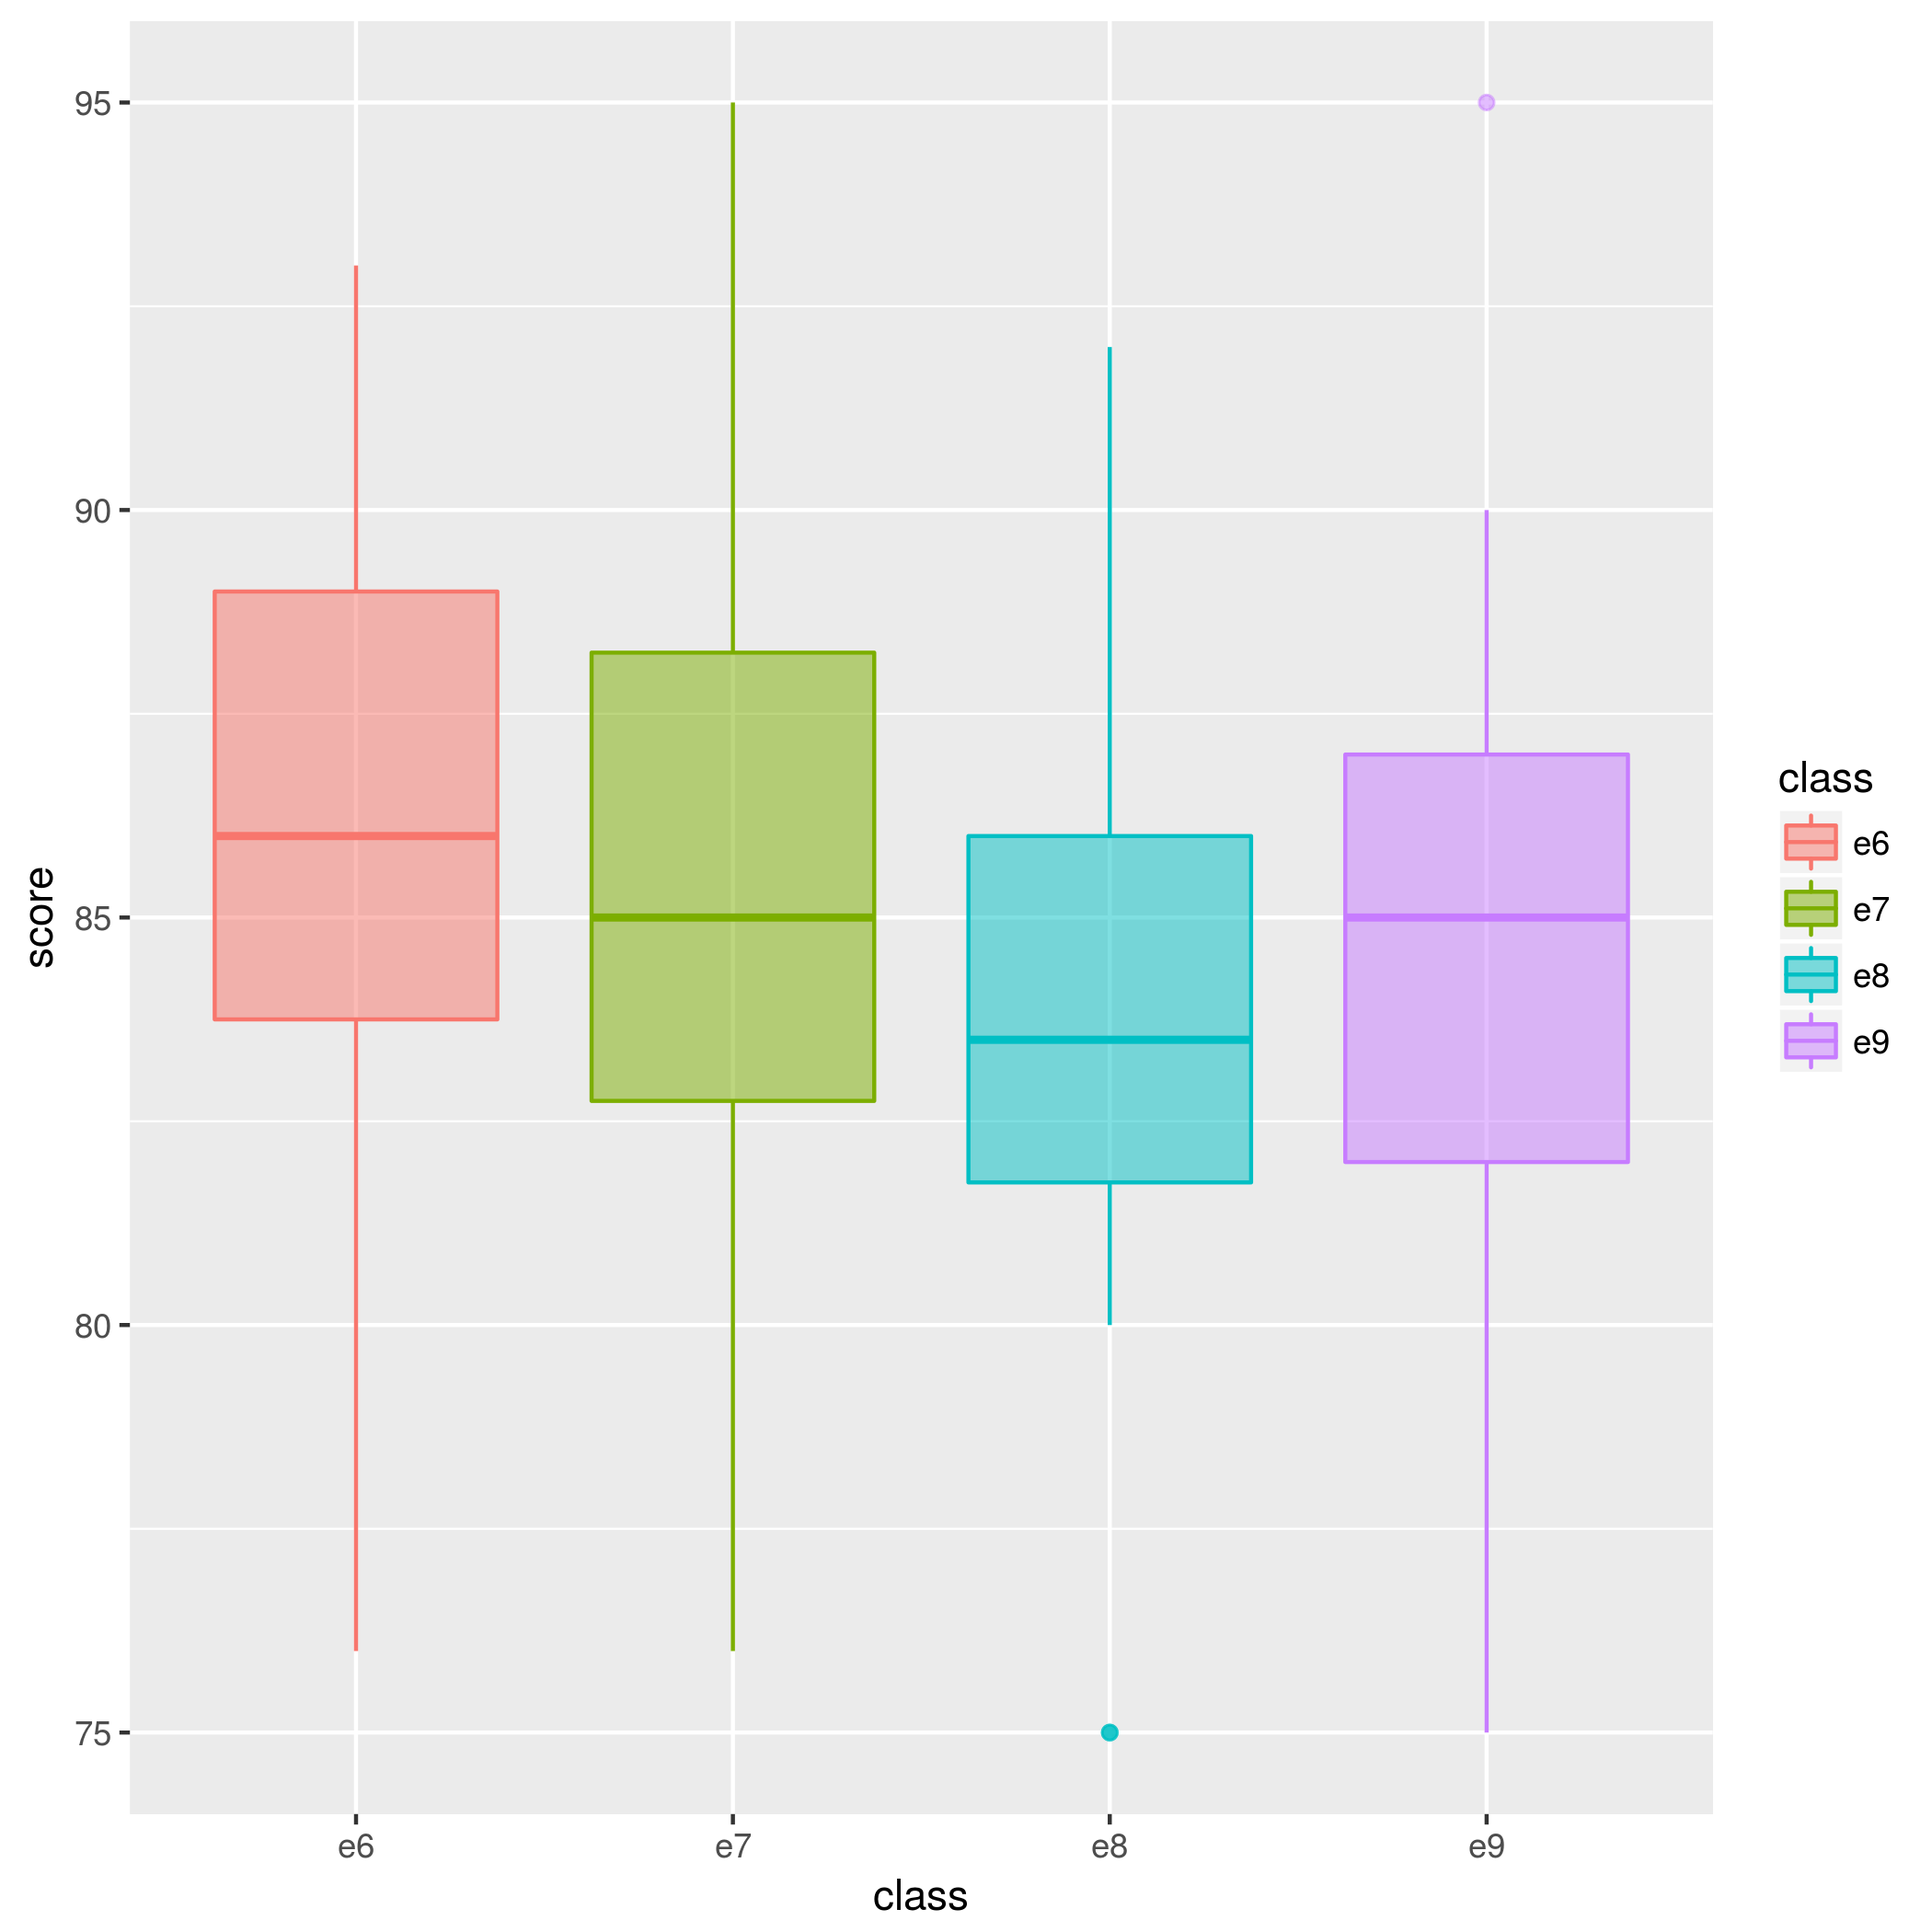
\includegraphics[width=0.65\textwidth]{c8.code.r.bp.png}
  \end{figure}
\end{frame}

\begin{frame}[fragile]
  \frametitle{扩展知识 | example | R}
\begin{lstlisting}[language=r]
gl <- ggplot(score_long2, aes(class, score, group=id2))
gl <- gl + geom_point()
gl <- gl + geom_line(aes(color=id2))

ggsave("id_lineplot.png", gl)
\end{lstlisting}
\end{frame}

\begin{frame}
  \frametitle{扩展知识 | example | R | plot}
  \begin{figure}
    \centering
    \includegraphics[width=0.65\textwidth]{c8.code.r.lp.png}
  \end{figure}
\end{frame}

\begin{frame}[fragile]
  \frametitle{扩展知识 | example | R}
\begin{lstlisting}[language=r]
lm_eqn <- function(df) {
  m <- lm(final ~ exp, df)
  eq <- substitute(italic(y) == a + b %.% italic(x) *","* ~~italic(r)~"="~r1 *","* ~~italic(R)^2~"="~r2, 
                   list(a = format(coef(m)[1], digits=2), 
                        b = format(coef(m)[2], digits=2), 
                        r1 = format(sqrt(summary(m)$r.squared), digits=3),
                        r2 = format(summary(m)$r.squared, digits=3)))
  as.character(as.expression(eq))
}
\end{lstlisting}
\end{frame}

\begin{frame}[fragile]
  \frametitle{扩展知识 | example | R}
\begin{lstlisting}[language=r]
score_wide2 <- score_wide %>% group_by(id,name,final) %>% summarise(exp=mean(c(e6,e7,e8,e9))) 

gr <- ggplot(score_wide2, aes(exp, final))
gr <- gr + geom_point()
gr <- gr + geom_smooth(method="lm", color="red", formula=y~x)
gr <- gr + geom_text(x=82, y=100, label=lm_eqn(score_wide2), parse=TRUE, size=5, color="blue")

ggsave("correlation_plot.png", gr)
\end{lstlisting}
\end{frame}

\begin{frame}
  \frametitle{扩展知识 | example | R | plot}
  \begin{figure}
    \centering
    \includegraphics[width=0.65\textwidth]{c8.code.r.cor.01.png}
  \end{figure}
\end{frame}

\begin{frame}[fragile]
  \frametitle{扩展知识 | example | R}
\begin{lstlisting}[language=r]
id1 <- score_wide2[which.min(score_wide2$final),]$id
score_wide3 <- score_wide2 %>% filter(id!=id1)

gr2 <- ggplot(score_wide3, aes(exp, final))
gr2 <- gr2 + geom_point()
gr2 <- gr2 + geom_smooth(method="lm", color="red", formula=y~x)
gr2 <- gr2 + geom_text(x=82, y=100, label=lm_eqn(score_wide3), parse=TRUE, size=5, color="blue")

ggsave("correlation_plot_correct.png", gr2)
\end{lstlisting}
\end{frame}

\begin{frame}
  \frametitle{扩展知识 | example | R | plot}
  \begin{figure}
    \centering
    \includegraphics[width=0.65\textwidth]{c8.code.r.cor.02.png}
  \end{figure}
\end{frame}


\input{snippet/class_tail.tex}
